\chapter{Background}
\label{chapter2}
Although transmitted wave-forms begin as well defined, man-made, synthetic structures, a virtually endless number of probabilistic, and sometimes non-linear, phenomenon alter the observed wave-forms receive-side~\cite{o2016radio}. Even within a single phenomenon, there can exist again a virtually endless number of variations of that imperfection from one wireless channel to another. Some of the most prevalent and common imperfections include:
\begin{enumerate}
	\item Additive white Gaussian noise, and information theory model used to mimic the effects of many wide-band noise sources
    \item Path loss reduction of signal power density due to refraction, diffraction, absorption, aperture-medium coupling loss, and free-space loss
    \item Doppler shifts resulting from motion of the transmitter, receiver, or scatterers and reflectors within the wireless channel
    \item Coupled noise resulting from inter-modulation, interference from same and adjacent channels, industrial noise, Cosmic and terrestrial events
	\item Carrier frequency offset of both the transmitter and receiver's local oscillators, which drive each radio's mixers
	\item Phase ambiguity introduced by the unknown distance between transmitter and receiver
	\item Random symbol timing offset resulting from independently running sample clocks
    \item IQ imbalance resulting from phase and magnitude mismatches between the sine and cosine sections of receiver and transmitter chains
    \item Rounding of sampled voltages and digital filter coefficients due to Quantization
    \item Electronic Noise caused by semi-conductors such as shot and flicker noise
\end{enumerate}
In this chapter, background information is given on classical channel model theory in Section~\ref{chanmods} to support Chapter~\ref{chapter3}. Training of Neural Networks is described in Section~\ref{training}, and in Section~\ref{modclass} a survey of modulation classification is discussed to support Chapter~\ref{chapter4}.

\section{Classical Channel Models}
\label{chanmods}
When a communications transmit-receive pair move information from one point to another, there is a great deal of sequential tasks that are performed by the transmit and receive chain of tasks (see Figure~\ref{fig:fulltxrx}). It is the goal of this section to describe popular models which discuss the impact of imperfections of these tasks, as well as perturbations introduced during the informations journey from sender to receiver. The first such model that is often discussed in this field is the model for Additive White Gaussian Noise (AWGN).

\begin{figure*}[ht!]
	\centering	\includegraphics[width=1\textwidth,keepaspectratio]{figs/txrxfull__1_.pdf}
    \caption{A flow chart of a transmit and receive chain of communications tasks. Arrows indicate movement of information from one block to another. The form that information takes at each step is communicated through annotations. Antennas are pictured as upside-down triangles.} 
\label{fig:fulltxrx}      
\end{figure*}

\subsection{Additive White Gaussian Noise (AWGN)}
\label{awgn}
As it will become apparent in this section, there is a virtually unending number of types and sources of noise in a wireless channel. The central limit theorem states that as independent random variables are added together, the more there are, the closer their joint distribution approaches a Gaussian probability density function (PDF):
\begin{equation}
\label{eq:gaussianpdf}
f_x(x) = \frac{1}{\sqrt{2\pi \sigma^2}} e^{-\frac{(x-\mu)^2}{2\sigma^2}}.
\end{equation}
AWGN is described as additive because it is added to any transmission, no matter its location. Additionally, there exists enough noise sources to approximate the CLT at all frequencies (see Figure~\ref{fig:awgn}) such that the noise has uniform power across the frequency band. This is why AWGN is described as white, it is an analogy for how white frequencies of optical wavelengths are the sum of all other colors of the visible light frequency band.

\begin{figure*}[ht!]
	\centering	\includegraphics[width=1\textwidth,keepaspectratio]{figs/awgn.png}
    \caption{A cartoon showing the sum of several Gaussian PDFs (\ref{eq:gaussianpdf}) at varying frequencies. Amplitude and location of PDFs are arbitrary and not representative of any measurement or formal model.} 
\label{fig:awgn}      
\end{figure*}

Claude Shannon proved in~\cite{Shannon} that the channel capacity $C$ of a wireless channel with power constraint $\frac{1}{k}\sum_{i=1}^k x_i^2 \leq P$ for $k$ message codewords $x_1, x_2,...,x_k$, is:
\begin{equation}
\label{eq:capacity}
C = \frac{1}{2} \log_2 \bigg(1+\frac{P}{N}\bigg),
\end{equation}
where $N$ is the wireless channel AWGN variance. Codewords make up a codebook, or all possible messages sent. Consider the optical telegraph, a mid-1700's invention of the French Chappe brothers. Five brightly colored panels are painted onto a board and hidden by shutters that can be either open (1) or closed (0), conveying $2^5=32$ messages, $x \in \{1,0,0,0,0 \}, \{0,1,0,0,0 \},...,\{1,1,1,1,1 \}$. The larger the number and dimensionality of codewords, the larger the power constraint $P$, the larger the channel capacity $C$. 

\subsection{Path Loss}
\label{pathloss}
A key contributer to SNR is the received power, $P_r$. According to the Friis formula, the received power can be calculated in dBm as:
\begin{equation}
\label{eq:friis}
P_r = P_t + G_t + G_r + 20\log_{10}\bigg(\frac{\lambda}{4\pi d}  \bigg),
\end{equation}
where $P_t$ is the transmitted power, $G_r, G_t$ are the receiver and transmit antenna gains, $\lambda$ is the wavelength of the transmitted signal, and $d$ is the transmission distance. The formula has a few assumptions: far-field transmission ($d \gg \lambda$), the signal is narrow-band, and antennas are isotropic in the direction of transmission. Notice that power received decreases with both increased frequency and distance.

This section will discuss the relationship between received power and distance between transmitter and receiver of both wide-band and narrow-band signals. A narrow-band signal's bandwidth does not significantly exceed the coherence bandwidth of the channel the signal is traveling through. A received signal is considered significantly wide if the inverse of the channel's root mean squared (rms) delay spread $\tau_{rms}$:
\begin{equation}
\label{eq:trms}
\tau_{rms} = \sqrt{\overline{\tau^2}+(\overline{\tau})^2},
\end{equation}
is five times smaller than the signal's bandwidth~\cite{pahlavan2005wireless}.
\begin{equation}
\label{eq:cohbw}
\frac{5}{\tau_{rms}} < BW.
\end{equation}
The delay spread $\overline{\tau^n}$ is defined as
\begin{equation}
\label{eq:tau}
\overline{\tau^n} = \frac{\sum_{i=1}^L \tau_i^n |\beta_i|^2}{\sum_{i=1}^L |\beta_i|^2},
\end{equation}
where the additional time required for the $ith$ signal path, or ray, to arrive is $\tau_i$, and the power of the $ith$ ray is $|\beta_i|^2=A_0 a_i/d_i$. The path distance of the $ith$ ray is $d_i$, the overall reflection coefficient of the $ith$ ray is:
\begin{equation}
\label{eq:coeff}
a_i = \sum_{j=1}^{K_i} a_{ij},
\end{equation}
where $a_{ij}$ is one of $K_i$ reflections for the $ith$ ray. $A_0 = \sqrt{P_0}$, the power of the received signal from one meter away:
\begin{equation}
\label{eq:po}
P_0 = P_tG_rG_t(\lambda/4\pi)^2.
\end{equation}

A popular model for representation of a channel with path loss is the discrete delay channel model~\cite{pahlavan2005wireless} (see Figure~\ref{fig:discdelay}). However, this model behaves differently for narrow and wide-band signals.
\begin{figure*}[ht!]
	\centering	\includegraphics[width=1\textwidth,keepaspectratio]{figs/discdelaychannel.png}
    \caption{The discrete delay channel model. Inputs each have isolated time delays $\tau_i$, ray powers $|\beta_i|^2=A_0 a_i/d_i$, and ray phases $e^{j\phi_i}$.} 
\label{fig:discdelay}      
\end{figure*}

\subsubsection{Narrow-Band Signal}
A signal is determined to be narrow-band using (\ref{eq:cohbw}), the received power can be formulated as:
\begin{equation}
\label{eq:prnarrow}
P_r = P_0 \Bigg| \sum_{i=1}^L \frac{a_i}{d_i} e^{j\phi_i} \Bigg|
\end{equation}
where the received phase offset $\phi_i=-2\pi d_i/\lambda$. Notice how the phase of each ray $e^{j\phi_i}$ has the potential to add both constructively and destructively (see Figure~\ref{fig:narrowpower}).
\begin{figure*}[ht!]
	\centering	\includegraphics[width=1\textwidth,keepaspectratio]{figs/narrowbandpower.png}
    \caption{A series of narrow-band transmissions from~\cite{pahlavan2005wireless}, received in a room obtained by the 2D ray-tracing model (\ref{eq:prnarrow}). a) Line of Sight (LOS) path (no reflections). b) First-order reflection ($K=2$ for coefficients equation (\ref{eq:coeff})). c) Second-order reflection, $K=3$. d) Third-order reflection, $K=4$. Notice that higher order reflections have higher frequency changes in power received as distance increases, and that the average power (black line) decreases with distance due to (\ref{eq:friis}).} 
\label{fig:narrowpower}      
\end{figure*}

\subsubsection{Wide-Band Signal}
A wide-band signal in the frequency domain can be shown to be of a short time duration in the time domain~\cite{rappaport1996wireless}. Often these bursts of signals are modeled as impulses, $\delta (t)$. In ideal wide-band communications, each path of arrival an impulse makes from transmitter to receiver are isolated. Additionally, since impulse's duration are instantaneous compared to time delays $\tau_i$, the phase offset of each ray does not add constructively or destructively. Consequentially, and similarly to (\ref{eq:prnarrow}), the received power of a wide-band signal can be formulated as~\cite{pahlavan2005wireless}:
\begin{equation}
\label{eq:prwide}
P_r = P_0 \Bigg| \sum_{i=1}^L \frac{a_i}{d_i} \Bigg| = \sum_{i=1}^L |\beta_i|^2,
\end{equation}
with the phase term $e^{j\phi_i}$ missing. The result is that wide-band path loss doesn't vary from (\ref{eq:friis}) very much, unlike Figure~\ref{fig:narrowpower}. For a series of wide-band path loss experiments, see Figure~\ref{fig:widepower}.
\FloatBarrier
\begin{figure*}[ht!]
	\centering	\includegraphics[width=1\textwidth,keepaspectratio]{figs/widebandpower.png}
    \caption{A series of wide-band transmissions from~\cite{pahlavan2005wireless}, received in a room obtained by the 2D ray-tracing model (\ref{eq:prnarrow}). a) Line of Sight (LOS) path (no reflections). b) First-order reflection ($K=2$ for coefficients equation (\ref{eq:coeff})). c) Second-order reflection, $K=3$. d) Third-order reflection, $K=4$. Average power (black line) decreases with distance due to (\ref{eq:friis}). For higher order reflections the power received is higher because the impulse signals are not totally isolated.} 
\label{fig:widepower}      
\end{figure*}
\FloatBarrier

\subsubsection{Knife-Edge Diffraction Model}
A popular method used to modify (\ref{eq:friis}) is the knife-edge diffraction model~\cite{rappaport1996wireless}. Given the transmitter (see Figure~\ref{fig:knifeedge}) $\Upsilon$ receiver $R$, obstruction of height $h$ above the direct path from $\Upsilon$ to $R$, and distances $d_1, d_2$ from the transmitter and receiver to the obstruction, respectively, the Fresnel-Kirchoff diffraction parameter can be calculated as:
\begin{equation}
\label{eq:v}
v = h\sqrt{\frac{2(d_1+d_2)}{\lambda d_1 d_2}},
\end{equation}
to estimate the additional gain to free space (\ref{eq:friis}) as:
\begin{equation}
\label{eq:diffraction}
G_{dB} = 20 \log |F(v)|,
\end{equation}
where the Fresnel integral can be calculated as:
\begin{equation}
\label{eq:fresnel}
F(v) = \frac{(1+j)}{2} \int_v^{\infty} e^{(-j\pi t^2)/2} dt.
\end{equation}
While it is often sufficient~\cite{rappaport1996wireless} to model just the largest diffraction, there are situations where a multiple knife-edge diffraction model would increase the accuracy of a path loss model significantly. 
\begin{figure*}[ht!]
	\centering	\includegraphics[width=0.8\textwidth,keepaspectratio]{figs/knifeedge.png}
    \caption{An illusration~\cite{rappaport1996wireless} of (\ref{eq:diffraction}), where $\Upsilon$ is the transmitter, $R$ is the receiver, $h$ is the height of the obstruction starting from the direct path from $\Upsilon$ to $R$, and $d_1, d_2$ from the transmitter and receiver to the obstruction, respectively. The Huygens secondary source mimics a potentially strong reflected path, often taking the form of a reflection off a layer of the earth's ionosphere (see Section~\ref{terrestrial}).} 
\label{fig:knifeedge}      
\end{figure*}
\subsubsection{Topographical Path Loss Models}
For high power, long range transmissions of frequencies up to L-band (2000 MHz) from a tall base-station tower to a mobile user, the most popular path loss model to be used in the free space Friis formula (\ref{eq:friis}) is the Okumara-Hat~a\cite{oku68} empirical path loss model, whose behavior was collected in Tokyo, Japan using isotropic antennas, and has seen widespread use. The formula is rated for use up to 100 km and for at least 1 km, and is rated for a base-station height up to 200 m and a mobile receiver height of up to 3 m. Over the years, many measurement campaigns~\cite{tsb88tia} have been conducted to expand the range of distances and frequencies the model can accommodate. The original Okumara model can be described~\cite{rappaport1996wireless} as use of the Friis formula (\ref{eq:friis}) where $L_{path}$ is instead:
\begin{equation}
\label{eq:okuhata}
L_{50, dB}  = L_F + A_{mu}(f,d) - G(h_{te})-G(h_{re})-G_{AREA},
\end{equation}
where $L_{50, dB}$ is the 50th percentile (mean) of the propagation loss, $L_F$ is the free space propagation loss, $A_{mu}(f,d)$ is the median attenuation relative to free space (see Figure~\ref{fig:okumara}), $G(h_{te}), G(h_{re}$ are the transmitting and receiving antenna gain factors (\ref{eq:antgain}), respectively, and $G_{AREA}$ is the gain with respect to the type of environment (see Figure~\ref{fig:garea}).

\begin{figure*}[ht!]
	\centering	\includegraphics[width=0.6\textwidth,keepaspectratio]{figs/garea.png}
    \caption{A plot~\cite{rappaport1996wireless} of correction factor, $G_{AREA}$ to be used in (\ref{eq:okuhata}) for various frequencies in open, quasi-open, and suburban areas (urban not listed).} 
\label{fig:garea}      
\end{figure*}

\begin{figure*}[ht!]
	\centering	\includegraphics[width=0.6\textwidth,keepaspectratio]{figs/okumara.png}
    \caption{A plot~\cite{rappaport1996wireless} of $A_{mu}(f,d)$, the median attenuation relative to free space, used in (\ref{eq:okuhata}). Plot assumes base-station height $h_t=200 m$, mobile receiver height $h_r=3 m$, an Urban area, and various distances and frequencies.}
\label{fig:okumara}      
\end{figure*}

For various antenna heights, the antenna gain factors can be described as:
\begin{subequations}
\label{eq:antgain}
\begin{align}
\begin{array}{cc}
G(h_{te}) = 20\log \big( \frac{h_{te}}{200} \big), & 1000 m > h_{te} > 30m 
\end{array}
\\
\begin{array}{cc}
G(h_{re}) = 10\log \big( \frac{h_{re}}{3} \big), & h_{re} \leq 3 m
\end{array}
\\
\begin{array}{cc}
G(h_{re}) = 20\log \big( \frac{h_{re}}{3} \big), & 10 m > h_{re} > 3 m.
\end{array}
\end{align}
\end{subequations}


\subsubsection{Just the Beginning: Fading}
Path loss ideas visited in this section have just surveyed the most popular models. How do these models change in a wireless channel over time? A host of path loss and fading (or shadowing) models exist for high and low altitude antennas of high and low frequency transmissions over short and large distances with narrow and wide bandwidths in both LOS and NLOS situations~\cite{tsb88tia,rappaport1996wireless,pahlavan2005wireless}. An exhaustive list of industry standard models can be found in~\cite{tsb88tia}. Fading is a term used to describe variations in the path loss of a system over time, and can be broken into two categories: fast-fading ($1/D_S$ large (\ref{eq:doppspread})) and slow-fading ($1/D_S$ small (\ref{eq:doppspread})). Sources of slow-fading include large obstructions such as mountains, seasonal changes to the ionosphere (see Section~\ref{terrestrial}), and any gradual change to the wireless channel such as urban construction.  Fast-fading sources include weather changes, activity in the earth's ionosphere (see Section~\ref{terrestrial}), solar flares, and any rapid changes to the wireless channel.

\subsection{Doppler Shift}
In practice, information is often sent in a radio system under mobile conditions. The impacts of this can be considerable, especially in satellite and railway communications. Consider a sine wave being transmitted via a radio link in a mobile environment, as in Figure~\ref{fig:mobil_illust}.

\FloatBarrier
\begin{figure*}[ht!]
	\centering	\includegraphics[width=1\textwidth,keepaspectratio]{figs/doppler_graphic.png}
    \caption{An illustration~\cite{pahlavan2005wireless} of a radio link between a moving transmitter (left) and stationary receiver (right). Transmitter is moving at velocity $V_m$ at an instantaneous distance $d_0$ from the receiver.} 
\label{fig:mobil_illust}      
\end{figure*}
\FloatBarrier

As the transmitter moves towards the receiver, the instantaneous distance $d_0$ will shrink, impacting transmission time as a function of time,
\begin{equation}
\label{eq:delayt}
\tau(t) = \tau_0 - \frac{V_m}{c}t,
\end{equation}
where $c$ is the speed of light in free-space, 3e8 m/s, and $\tau_0=d_0/c$ is the starting transmission time. Given this, the transmitted sine wave can be formulated by Euler's formula as:
\begin{equation}
\label{eq:doppsig}
r(t) = A_r e^{j2\pi f_c [t - \tau(t) ]} = A_r e^{j[2\pi (f_c+f_d)t-\phi ]},
\end{equation}
where $f_c$ is the sine waves carrier frequency, $A_r$ is the amplitude of the received signal, $\phi=2\pi f_c tau_0$ is the current phase offset, and $f_d$ is the Doppler shift caused by movement,
\begin{equation}
\label{eq:doppler}
f_d = \frac{V_m}{c} f_c \cos(\theta),
\end{equation}
where $\theta$ is the direction of movement, for zero degrees being moving straight towards the receiver. This frequency shift is observed by the receiver, positive or negative depending on the direction of movement, where magnitude is maximized by the cosine when moving exactly toward or away from the transmitter. Commonly these maximal outcomes of (\ref{eq:doppler}) are described as the maximum Doppler shift $f_M = \pm \frac{V_m}{c} f_c$ of bandwidth $B_D = 2f_M$.

However, as shown in Section~\ref{pathloss}, rarely is there one ray (see Figure~\ref{fig:discdelay}) in a wireless channel. Each ray is effected differently, and as consequence the frequency domain representation of the signal is affected by a Doppler spectrum, or spread $D(\lambda)$, derived as follows: consider the wireless channel responding to probing impulse responses $\delta(t)$ at time delays $\tau$ in the form $h(\tau, t)$, where for the input $x(t)$, the channel output is $y(t) = x(t) \circledast h(t)$.
\begin{equation}
\label{eq:multipathimpulse}
h(\tau, t) = \sum_{i=1}^L \beta_i e^{j\phi_i} \delta(t-\tau_i),
\end{equation}
The autocorrelation the observed impulse response at two different delays and times can then be formulated as~\cite{pahlavan2005wireless}:
\begin{equation}
\label{eq:Rhh}
R_{hh}(\tau_1,\tau_2;t_1,t_2) = R_{hh}(\tau_1;\Delta t) \delta(\tau_1-\tau_2),
\end{equation}
for $\Delta t = t_2-t_1$. Given $R_{hh}$, the autocorrelation in the frequency domain given the time-varying frequency domain impulse response $H(f;t)=\int_{-\infty}^{\infty} h(\tau;t) e^{-j\omega \tau}d\tau$ is formulated in~\cite{pahlavan2005wireless} as:
\begin{equation}
\label{eq:RHh}
R_{Hh}(f_1,f_2; \Delta t) = R_{Hh}(\Delta f; \Delta t),
\end{equation}
where $\Delta f = f_2-f_1$ and the channel is assumed to have Wide-Sense Stationary Uncorrelated Scattering (WSSUS), which is valid for most wireless channels~\cite{pahlavan2005wireless}, and implies that the signal variations on paths of different delays $\tau_i$ are uncorrelated, and the correlations between paths of equal delays are stationary, or time-invariant. Additionally, the autocorrelation can be estimated as $R_{Hh}(\Delta f)$ if the channel is slowly time-varying or time-invariant.

Finally, we can derive the Doppler spectrum $D(\lambda)$ using the Fourier transform of (\ref{eq:RHh}):
\begin{equation}
\label{eq:RHH}
R_{HH}(\Delta f; \lambda) = \int_{-\infty}^{\infty} R_{Hh}(\Delta f; \Delta t) e^{-j2\pi \lambda \Delta t}d(\Delta t),
\end{equation}
as:
\begin{equation}
\label{eq:doppspect}
D(\lambda) = R_{HH}(0;\lambda).
\end{equation}
The spectrum is limited by $\pm f_M$ (\ref{eq:doppler}), and the amount of variation of the spectrum over frequency is described by the Doppler spread:
\begin{equation}
\label{eq:doppspread}
B_{D,rms}^2 = \frac{\int_{-f_M}^{f_M} \lambda^2 D(\lambda) d\lambda}{\int_{-f_M}^{f_M} D(\lambda) d\lambda}.
\end{equation}
Equations (\ref{eq:Rhh}) through (\ref{eq:RHH}) are summarized in Figure~\ref{fig:doppflow}.

\begin{figure*}[ht!]
	\centering	\includegraphics[width=0.6\textwidth,keepaspectratio]{figs/doppler_flow.png}
    \caption{A flow chart~\cite{pahlavan2005wireless} summarizing equations (\ref{eq:Rhh}) through (\ref{eq:RHH}). Arrows indicate Fourier (down) and inverse Fourier (up) transforms.} 
\label{fig:doppflow}      
\end{figure*}
In the most basic multi-path case, (\ref{eq:doppspect}) takes the form
\begin{equation}
\label{eq:jakes}
D(f) = \frac{1}{2\pi f_m} \bigg[1-\bigg(\frac{f}{f_m}^2 \bigg)  \bigg]^{-1/2}, |f| \leq f_m,
\end{equation}
or Jakes Doppler spectrum, where (\ref{eq:doppler}) is assumed and can be plotted over normalized frequency as seen in Figure~\ref{fig:jakes}.

\FloatBarrier 
\begin{figure*}[ht!]
	\centering	\includegraphics[width=0.6\textwidth,keepaspectratio]{figs/jakes.png}
    \caption{Jakes Doppler spectrum~\cite{pahlavan2005wireless} for a non-line-of-sight (a) and line-of-sight (b) transmission. Horizontal axis is normalized frequency, and frequency offset is maximal at $\pm f_M$, or movement directly away from and towards the receiver. The impulse in (b) indicates the Doppler shift associated with the line-of-sight ray.} 
\label{fig:jakes}      
\end{figure*}
\FloatBarrier
However, there is a whole field dedicated to modeling unique cases of Doppler shift. Some common cases in addition to Figure~\ref{fig:jakes} are displayed in Figure~\ref{fig:dopplers}.

\FloatBarrier
\begin{figure*}[ht!]
	\centering	\includegraphics[width=0.615\textwidth,keepaspectratio]{figs/dopplers.png}
    \caption{A series of impulse responses (\ref{eq:multipathimpulse}) and their Fourier transforms~\cite{pahlavan2005wireless}. (a) shows a LOS experiment using a stationary radio transmit-receive pair in a stationary environment ($B_D=0 Hz$ see (\ref{eq:doppspread})). (b) display results of LOS experiment using a stationary receiver, but mobile transmitter that moved randomly within a 12 meter radius of a fixed point, simulating a mobile user pacing on their telephone ($B_D=4.9 Hz$). (c) display results of an obstructed LOS (OLOS) experiment using stationary devices 4 meters apart, but with heavy pedestrian traffic around the transmitter ($B_D=5.7 Hz$). (d) display an OLOS experiment with stationary devices, but the transmitter is rotated at a rate of 2.5 rotations per second ($B_D=5.2 Hz$).}
\label{fig:dopplers} 
\end{figure*}
\FloatBarrier

\subsection{Coupled Noise}
test
\subsubsection{Inter-modulation}
\subsubsection{Crosstalk}
\subsubsection{In-Band Interference}
\subsubsection{Terrestrial Interference}
\label{terrestrial}
\subsubsection{Industrial Noise}
\subsubsection{Cosmic Noise}
There are numerous electromagnetic sources throughout the universe whose emissions travel very well through the vacuum of space and disturb radio transmissions. Cosmic noise is a categorical term that embodies various forms of noise, most commonly encountered at frequencies above 30 MHz~\cite{cosmic}:
\begin{itemize}
\item Receivers pointed towards nearby stars such as our sun, super massive black holes at the center of galaxies, and quasars.
\item Charged particles and meteorites that fall into the earth's orbit are deflected by the fundamental electro-mechanical Lorentz force due to the earth's magnetic field. This process produces Synchrotron radiation~\cite{cosmic} of emitted power $P \sim m^{-4}$, which results in most all radiation resulting from electrons and positrons due to their small mass. Synchrotron radiation is phase coherent for showers of large side surface area smaller than wavelengths emitted. Pulse amplitude is then defined~\cite{cosmic} as:
\begin{equation}
\label{eq:synchrad}
A \sim E_p e^{-\frac{r}{r_0}},
\end{equation}
where $E_p$ is the energy in Joules of the primary particle, $r$ is the distance to the shower core, and $r_0$ is an experimentally determined constant.
\item Super wide band noise generated by Cosmic Microwave Background Radiation (CMBR), a form of radiation persisting from the big bang, which is present homogeneously throughout the known universe (see Figure~\ref{fig:cmbr}).
\end{itemize}

\FloatBarrier
\begin{figure*}[ht!]
	\centering	\includegraphics[width=0.8\textwidth,keepaspectratio]{figs/cmbr.png}
    \caption{A plot~\cite{cmbr} of the intensity of the CMBR over frequency.} 
\label{fig:cmbr}      
\end{figure*}
\FloatBarrier

\subsection{Radio Front End}
The RFFE (see Figure~\ref{fig:fulltxrx}) is a term used to group all of the analog circuitry between a transmit or receive chain's antenna and mixer. At the most basic, RFFE's contain:
\begin{itemize}
\item A Band Pass Filter (BPF), used to pass through the expected signal at the expected carrier frequency and block out all other signals and noise. In-band noise and interference is still present. BPFs can also damage signals due to in-band ripple, and are vulnerable to thermal noise, shot noise, and transit-time noise (see Section~\ref{enoise}).
\item A Low-Noise Amplifier (LNA), used to increase the power of in-band signals above the noise floor. LNAs must have a low noise figure (NF), and are often only needed at frequencies above 30 MHz due to the increased path loss (\ref{eq:friis}).
\item A Local Oscillator (LO) in a RFFE drives the modulation and demodulation tasks by creating a carrier cosine wave-form. Phase noise (see Section~\ref{enoise}) can be introduced by 1/f noise, and the frequency of the carrier can drift with time (see Section~\ref{cfo}).
\item a Mixer, which combines the carrier wave-form with the transmitted or received wave-form to form the base-band signal or the Intermediate Frequency (IF) signal.
\end{itemize}

Besides the issues listed above, the initial spacing between a transmit and receive radio can introduce an initial phase offset, introducing phase ambiguity (see Section~\ref{phaseam}) even after frequency correction is performed. Digital filters and the DAC/ADC (see Figure~\ref{fig:fulltxrx}) can introduce significant error to signals through quantization (see Section~\ref{quant}), and in the case of pulse-shaped (see Figure~\ref{fig:rrc}) wave-forms, symbol timing offset (STO) (see Section~\ref{sto}) can push bit error rates (BER) to their limits, 1/M (\ref{eq:mary}).

Furthermore, the cosine and sine paths of the RFFE (see Figure~\ref{fig:sinecosine}) experience phase and magnitude imbalances, resulting in stretched IQ plots (see Section~\ref{iq}).

Finally, various forms of electronic noise (see Section~\ref{enoise}) can impede SNR, sometimes significantly.
\subsubsection{Carrier Frequency Offset (CFO)}
\label{cfo}
Each radio system (see Figure~\ref{fig:fulltxrx}) has either a down-converter or an up-converter (see Figure~\ref{fig:mixer}), shifting the center frequency of the signal (see Figure~\ref{fig:upconv}) either up to the carrier frequency if transmitting or down to the base-band if receiving. 

\FloatBarrier
\begin{figure*}[ht!]
	\centering	\includegraphics[width=0.8\textwidth,keepaspectratio]{figs/mixer.png}
    \caption{An illustration~\cite{rappaport1996wireless} of the base-band signal $m(t)$ being up-converted to the intermediate frequency $f_c$ by a mixer, where the carrier wave-form $A_c cos(2\pi f_c t)$ is generated by a local oscillator, and in this case half of the signal's bandwidth is filtered out (see Figure~\ref{fig:upconv} for a double side-band plots of the base-band spectrum of $m(t)$ and the up-converted spectrum of a $S_{DSB}(t)$.} 
\label{fig:mixer}      
\end{figure*}

This conversion, however, is not perfect and is often affected by both a phase offset (see Section~\ref{enoise}) and a frequency offset, the latter of which can modeled at each local oscillator as:
\begin{equation}
\label{eq:fo}
f_{o,max} = \frac{f_c \times PPM}{10^6},
\end{equation}
where $PPM$ is the parts per million resolution of the LO, often listed in a radio's user manual, $f_c$ is the carrier frequency, and $f_{o,max}$ is the maximum possible negative or positive frequency offset. For a transmit receive pair, the total offset can then be defined as $f_{o_1} + f_{o_2}$, where each offset is a Gaussian random variable bounded by each radio's $f_{o,max}$, making the random variable no longer Gaussian. This results in a minimum possible offset of zero cycles when each offset is zero or equal and opposite, or a maximum offset of $\pm 2 \times f_{o,max}$.


\begin{figure*}[ht!]
	\centering	\includegraphics[width=0.8\textwidth,keepaspectratio]{figs/upconv.png}
    \caption{A plot~\cite{rappaport1996wireless} of (a) the base-band magnitude spectrum $|M(f)|$ of $m(t)$ (see Figure~\ref{fig:mixer}), and (b) its up-converted double side-band magnitude spectrum $|S_{AM}(f)|$.}
\label{fig:upconv}      
\end{figure*}
\FloatBarrier

\subsubsection{Phase Ambiguity}
\label{phaseam}
As seen in Figure~\ref{fig:narrowpower}, the received phase offset $\phi_i = -2\pi d_i / \lambda$ can have significant effects on path loss. However, this issue goes much deeper than received power: when a demodulator (see Figure~\ref{fig:fulltxrx}) maps a base-band waveform from IQ points to bits, this phase offset rotates the constellation by an amount that has been found experimentally~\cite{pahlavan2005wireless} to be random according to the uniform distribution $\mathcal{U}(0,2\pi)$ radians. Consequently, constellation plots like Figure~\ref{fig:qpskconst} can become very ambiguous, where the plot could be flipped along the real or imaginary axis and still look identical. As a result, various forms of precautions have been developed to avoid errors resulting from phase ambiguity, including:
\begin{enumerate}
\item Equalization
\item Codewords
\item Differential Encoding
\end{enumerate}
\subsubsection{Symbol Timing Offset (STO)}
\label{sto}

\FloatBarrier
\begin{figure*}[ht!]
	\centering	\includegraphics[width=0.4\textwidth,keepaspectratio]{figs/email_ps.png}
    \caption{} 
\label{fig:stoin}      
\end{figure*}
\FloatBarrier

\FloatBarrier
\begin{figure*}[ht!]
	\centering	\includegraphics[width=0.4\textwidth,keepaspectratio]{figs/email_ifilt.png}
    \caption{} 
\label{fig:stoin}      
\end{figure*}
\FloatBarrier

\FloatBarrier
\begin{figure*}[ht!]
	\centering	\includegraphics[width=0.4\textwidth,keepaspectratio]{figs/email_comparison.png}
    \caption{} 
\label{fig:stoin}      
\end{figure*}
\FloatBarrier

\FloatBarrier
\begin{figure*}[ht!]
	\centering	\includegraphics[width=1\textwidth,keepaspectratio]{figs/stoiq.png}
    \caption{} 
\label{fig:stoin}      
\end{figure*}
\FloatBarrier

\subsubsection{IQ Imbalance}
\label{iq}
The transmit and receive chains of a radio system (see Figure~\ref{fig:fulltxrx}) contain a similar modulation (see Figure~\ref{fig:sinecosine}) and demodulation operations. The magnitude and phase seen by the cosine (in-phase) and sine (quadrature, 90 degrees out of phase) paths of these operations are often not perfectly matched in hardware implementations, resulting in a stretched IQ plot (magnitude imbalance) at the receiver before mapping to bits, or a situation where the I and Q axis are no longer perpendicular due to phase imbalance (I is not truly 0 degrees, Q is not truly -90 degrees). Quality instruments tend to keep this low, although it can vary to large amounts over frequency~\cite{n210sbx}. IQ imbalance can be modeled at mapping time for each symbol through the expression:
\begin{subequations}
\label{eq:iqimbal}
\begin{align}
sI = kI \times sI',
\\
sQ = -kQsin(\phi_{\epsilon}) \times sI' + kQcos(\phi_{\epsilon}) \times sQ',
\end{align}
\end{subequations}
where $sI', sQ'$ are the balanced in-phase and quadrature components of the symbol, $sI, sQ$ are the IQ imbalanced in-phase and quadrature components of the damaged symbol, $kI, kQ$ are the linear in-phase and quadrature gains, and $\phi_{\epsilon}$ is the phase difference between the two paths. Notice that for $\phi_{\epsilon} = 0$ and $kI=kQ=0$, IQ imbalance is not present, $sI=sI',sQ=sQ'$.

\FloatBarrier
\begin{figure*}[ht!]
	\centering	\includegraphics[width=0.8\textwidth,keepaspectratio]{figs/sinecosine.png}
    \caption{An illustration~\cite{rappaport1996wireless} of the in-phase and quadrature paths of the modulator block in a RFFE (see Figure~\ref{fig:fulltxrx}). The signals $\dot{m}(t), m(t)$ may not experience the same gains or appropriate phases of 0 and 90 degrees (\ref{eq:iqimbal}).} 
\label{fig:sinecosine}      
\end{figure*}
\FloatBarrier

\subsubsection{Quantization}
\label{quant}
A radio system (see Figure~\ref{fig:fulltxrx}) experiences numerous forms of approximations of infinite-resolution analog values~\cite{quant}. Two such examples are the digital approximations of analog wave-forms by the ADC, and the floating-point approximation of IIR filter coefficients (16, 32, or 64 bit typically). While a received wave-form has an infinite-resolution amplitude value, computers only have so much computational power and must reduce the value of voltages and and filter coefficients to so many points of precision (see Figure~\ref{fig:quant}).

\FloatBarrier
\begin{figure*}[ht!]
	\centering	\includegraphics[width=1\textwidth,keepaspectratio]{figs/quant.png}
    \caption{Three plots~\cite{quant} describing an example of the effects of quantization error on a section of a ramp signal, (left) sine wave, (middle) and noisy wave-form (right). These plots have a digital resolution of one, all wave-forms can only be represented by a zero value, one, two, or three.} 
\label{fig:quant}      
\end{figure*}
\FloatBarrier

\subsubsection{Electronic Noise}
\label{enoise}
\begin{enumerate}
	\item Thermal Noise, or Johnson-Nyquist noise, is a form of white noise (see Section~\ref{awgn}) that results from the agitation brought on by any applied voltage to the charge-carrying electrons inside a radio's conductive components of its RFFE (see Figure~\ref{fig:fulltxrx}). For a circuit with resistance $R$ in Ohms, a signal of bandwidth $\Delta f$ in Hertz generates an rms voltage of:
\begin{equation}
\label{eq;thermnoise}
v = \sqrt{4 k_B T R \Delta f},
\end{equation}
where $k_B=1.38 \times 10^{-23} J/K$ is Boltzmann's constant, and $T$ is the temperature of the circuit in Kelvin. This voltage is white, or applied at all frequencies, adding the power
\begin{equation}
\label{eq:thermpower}
P_{dBm} = -174 + 10 \log_{10} (\Delta f),
\end{equation}
assuming room temperature, $T=298.15 K$.
    \item Shot Noise: The unit used to describe current, Amperes = Coulombs/Sec, describes an average rate of movement of charge past a constant point. Current is a flow of electrons with small random variations in the arrival rates of charge. This phenomenon is what is described as shot noise in electronics, and it is usually insignificant. However, at high frequencies and low temperatures, shot noise can overpower other forms of electronic noise such as thermal noise as the dominating source.
    
A form of white noise, shot noise power begins by modeling electron flow as a Poisson process, ultimately deriving power as:
\begin{equation}
\label{eq:shot}
P = \frac{1}{2} qI \Delta f R,
\end{equation}
where $q=1.602\times 10^{-19} C$ is the charge of an electron, $I$ is the average DC current flowing through the conductor, $\Delta f$ is the bandwidth of the signal in Hertz, and $R$ is the resistance of the circuit in Ohms.

    \item Flicker Noise, or 1/f noise, occurs in all electronic devices as a low-frequency phenomenon resulting from small changes, or flickers, in temperature changing the resistivity, and ultimately inducing a small voltage, in conductive, current carrying sections of the RFFE. In communications, low-frequency noise might not seem like an issue, but local oscillators mix up flicker noise to frequencies close to the carrier, which is called oscillator phase noise. Flicker noise is typically characterized by the corner frequency $f_c$ (typically several kHz, determined by which Field Effect Transistor (FET) the RFFE (see Figure~\ref{fig:fulltxrx}) uses), below which electronic noise is dominated by flicker noise, and above which is dominated by the various white band noise sources such as thermal and shot noise.
    
As an Infinite Impulse Response (IIR) filter of order $N$, flicker noise can be modeled by convolving time-domain samples with a filter defined by the numerator coefficient $\lambda$ and the denominator coefficients $\gamma_i$ are determined recursively as:
\begin{subequations}
\label{eq:flickerIIR}
\begin{align}
\lambda = \sqrt{2\pi f_{o}10^{L/10}},
\\
\gamma_i = (i-2.5) \frac{\gamma_{i-1}}{i-1},
\end{align}
\end{subequations}
where $f_{o}$ is the frequency offset in Hz, $L$ is the phase noise level in dBc/Hz compared to the carrier power, and the filter coefficient initialization begins with $\gamma_1 = 1$. An IIR filter is defined by these coefficients and input waveform $x[n]$ in the sample domain as:
\begin{equation}
\label{eq:IIRdef}
y[n] = \frac{1}{\gamma_1} (\lambda x[n] - \gamma_2 y[n-1] - ... - \gamma_i y[n-i+1]).
\end{equation}
    
    \item Burst Noise results from the summed voltage errors resulting from Gibb's phenomenon (see Figure~\ref{fig:gibbs}) on several discrete voltage signals changing state simultaneously. Gibb's phenomenon is a model used to describe how sharp features in time-domain signals require higher and more frequency components (perfectly square wave-forms would require an infinite number of frequencies including frequencies of infinite cycles/Sec), but due to limitations in hardware high frequency components may not be available and small errors can occur at signal edges. If the various triggers, states, and clocks used in RFFE's transition states at the same time, the sum of these Gibb's errors can exceed hundreds of mV.
    
\FloatBarrier
\begin{figure*}[ht!]
	\centering	\includegraphics[width=0.8\textwidth,keepaspectratio]{figs/gibbs.png}
    \caption{A section of a time-domain square wave-form formulated by summing cosines. While the states of the square wave-form aims to have values of negative and positive one, there are large deviations near high-definition edges, and small ripples in flat sections. If unlucky, these analog deviations can sum to mV values.}
\label{fig:gibbs} 
\end{figure*}
\FloatBarrier
    
    
    \item Transit-Time Noise is a high frequency noise that occurs in transistors. Transistors are gate-like semi-conductors used to many effects in a radio's RFFE (see Figure~\ref{fig:fulltxrx}), consisting of three nodes: a base, collector, and emitter. When the voltage at a transistor's base is large enough, current is allowed to flow from emitter to base, functioning as a switch. When this transit time from emitter to base is long compared to the period of the Alternating Current (AC) signal, issues arise in the form of transit-time noise, as the transistor is no longer being operated in its designed range. The noise will increase with frequency as the signal period becomes shorter compared to transit-time.
\end{enumerate}

\section{Training Deep Learning}
\label{training}
In order to better understand what makes deep learning training data valuable, this section communicates the basic concepts of linear classifiers and convolutional neural network classifiers. Knowing how the data is used is important in knowing what good data is.
\subsection{Linear Classification}
\label{linclass}
A linear classifier is the simplest form of machine learning that classifies signals that uses weights instead of storing all training signals in memory, like the nearest-neighbor or K-nearest-neighbor classifier. A linear classifier is comprised of two main parts: a score function that reduces raw data to $K$ class scores (where $K$ is the number of class categories), and a loss function, which is a metric that describes how closely a training signal's class scores match the ground truth.
\subsubsection{The Neuron Analogy}
The word neural in the term neural network is inspired by an analogy bridging the worlds of math and biology. The basic computational cell of brain is the neuron (see Figure~\ref{fig:sub:cell}), and its mathematical model (see Figure~\ref{fig:sub:neuron}) is very rough. In reality, dendrites perform non-linear, time-varying operations on signals coming in from axons~\cite{cs231} rather than the multiplication of a scalar, as seen in the mathematical model. Furthermore, there are many types of neurons, and a very important aspect of their behavior that is ignored in machine learning is the timing of their axon firings. 

\begin{minipage}[c]{0.5\textwidth}
   \begin{figure}[H]
      \centering
      \captionsetup{width=.9\linewidth}
      \includegraphics[width=\textwidth]{figs/cellneuron.png}
      \caption{An illustration~\cite{cs231} of a biological neuron. A neuron cell is composed of a nucleus which receives signals from many dendrites. The amount of influence a dendrite has on a neuron is determined by synapses. When the sum of incoming signals is above a threshold, the nucleus fires a signal down its axon, which in turn splits into many dendrites, feeding into other neurons.} 
      \label{fig:sub:cell}
   \end{figure}
\end{minipage}%
\begin{minipage}[c]{0.5\textwidth}
   \begin{figure}[H]
      \centering
      \captionsetup{width=.9\linewidth}
      \includegraphics[width=\textwidth]{figs/neuron_model.jpeg}
      \caption{A mathematical representation~\cite{cs231} of Figure~\ref{fig:sub:cell}. The previous neurons' axons carry the signals $x_0, x_1, x_2$, which split into many dendrites. Synapses influence that value by a weight, ($w_0, w_1, w_2$). The cell body adds weights to each incoming dendrite ($b_0, b_1, b_2$), computes the dot product of all dendrites, and outputs a signal on its axon defined as the output of some activation function $f$ whose input is the dot product.} 
      \label{fig:sub:neuron}
   \end{figure}
\end{minipage}


\subsubsection{Multi-class Support Vector Machine (SVM)}
The SVM is a commonly used loss function that wants the correct class for each signal to have a score higher than the wrong ones by a margin of $\Delta$. The SVM is defined as:
\begin{equation}
\label{eq:svm}
L_i = \sum_{j\neq y_i}max(0,S_j-S_{y_i}+\Delta),
\end{equation}
As an example, if the ground truth for the $ith$ signal used to train a three-class linear classifier is $y_i = 0 \neq 1 \neq 2$, the margin $\Delta = 10$, and the class scores $S = \lbrack 13, -7, 11 \rbrack$, 
\begin{subequations}
\label{eq:svmexample}
\begin{align}
L_i = max(0, S_1 - S_0 + \Delta) + max(0, S_2 - S_0 + \Delta),
\\
L_i = max(0, -7 - 13 + 10) + max(0, 11 - 13 + 10),
\\
L_i = max(0, -10), max(0, 8),
\\
L_i = 8.
\end{align}
\end{subequations}
The $j=1$ term contributes no loss to $L_i$ because the correct class score $S_0 = 13$ was more than $\Delta = 10$ larger than the incorrect score $S_1 = -7$. The $j=2$ term was not, so the loss score was increased by how much the margin was missed by, eight.

A commonly used reduction for the dot product of terms $Wx_i+b$ is to combine $W, b$ into one matrix. This is done by adding a unit value to the end of each flattened row vector signal $x_i$ as shown in Figure~\ref{fig:wb}.

\begin{figure*}[ht!]
	\centering	\includegraphics[width=1\textwidth,keepaspectratio]{figs/wb.jpeg}
\caption{An illustration~\cite{cs231} of reducing $W \in \lbrack 3,4 \rbrack$ and $b \in \lbrack 3,1 \rbrack$ into a single matrix, $W \in \lbrack 3,5 \rbrack$ by adding a unit value to the end of $x_i \in \lbrack 5,1 \rbrack$.} 
\label{fig:wb}      
\end{figure*}

For a single-layer Linear Classifier (input is directly connected to neurons which are directly used to calculate class scores) and linear score function $S = f(x_i,w)$, SVM can be vectorized and written as:

\begin{equation}
\label{eq:svmvector}
L_i = \sum_{j\neq y_i} max(0, w_j^Tx_i - w_{y_i}^Tx_i+\Delta),
\end{equation}

where each of the $N$ training signals $x_i, i=0,1,...,N-1$ are the flattened row vectors of two-dimensional ($D = 2$) signals, where each element represents an alternating in-phase and quadrature (IQ) sample. All flattened signals together make up the matrix of samples $x \in \lbrack N, k \times D \rbrack$.

Suppose we are given a new set of scores $S=\lbrack 13, -7, -5 \rbrack$, such that now in (\ref{eq:svmexample}) we achieve $L_i = 0$. If we set all weights $W = \lambda W$, for $\lambda = 3$, through (\ref{eq:svmvector}) we would achieve in (\ref{eq:svmexample}) $L_i = max(0, (-7-13)\lambda+10) + max(0, (-5-13)\lambda+10) = 0$. For any $\lambda>1$, in fact, the loss function would remain at zero. To keep weights minimal and remove this ambiguity, the SVM employs a regularization penalty, defined as:
\begin{equation}
\label{eq:regpen}
R(w)=\sum_k\sum_l w_{k,l}^2,
\end{equation}
such that the SVM is now defined as:
\begin{equation}
L_i = \sum_{j\neq y_i} max(0, w_j^Tx_i - w_{y_i}^Tx_i+\Delta) + \lambda\sum_k\sum_l w_{k,l}^2.
\end{equation}
This way, no single input dimension of a training example $x_i$ can have a dominating impact on all $K$ scores by itself. For example, the unit amplitude, two-symbol, two-SPS Quadrature Phase Shift Keying (QPSK) signal $x_i = \lbrack 1,1,1,1 \rbrack$ and two weight vectors $w_0 = \lbrack 1,0,0,0 \rbrack$ and $w_1 = \lbrack 0.25,0.25,0.25,0.25 \rbrack$ result in the same dot product $w_0^Tx_i=w_1^Tx_i=1$, but the regularization penalty for $R(w_0) = 1^2 + 0^2+0^2+0^2=1 > R(w_1)=0.25^2+0.25^2+0.25^2+0.25^2=0.25$. As a result, $w_1$ would achieve the lower regularization loss $\lambda R(w)$ and total loss $L_i$, because the influence of its weights are more evenly distributed across both the I and Q components of both the first and second symbol of the transmission $x_i$. Using $w_0$, all influence is given to the in-phase component of the first symbol. In~\cite{cs231}, it is suggested that $\Delta, \lambda$ can safely be set to one in all cases, and can be tuned together as a single hyper-parameter, a concept covered next in Section~\ref{valid}: Validation.

\subsubsection{Soft-Max Classifier}
The other popular loss function, besides SVM, is the soft-max classifier where the soft-max function is defined as $f_j(z)$ and its loss function $L_i$:

\begin{subequations}
\label{eq:softmax}
\begin{align}
f_j(z) = \frac{e^{z_j}}{\sum_k e^{z_k}},
\\
L_i = -\log \Bigg( \frac{e^{f_{y_i}}}{\sum_j e^{f_j}} \Bigg).
\end{align}
\end{subequations}
Where $f_j$ is the j-th element of the $K$ class scores $f_j, j=0,1,...,K-1$. This function can be though of as the normalized probability that the label $y_i$ is correct given the signal $x_i$, parameterized by weights matrix $W$ (\ref{fig:wb}):

\begin{equation}
\label{eq:probsoftmax}
P(y_i,x_i;W) = \frac{e^{f_{y_i}}}{\sum_j e^{f_j}}.
\end{equation}
The function is analogous to a probability in the sense that each soft-max rating $0 \leq f_j \leq 1$ and $\sum_j f_j = 1$. A three-class modulation linear classifier soft-max vector $f = \lbrack 0.2,0.2,0.6 \rbrack$, for instance, may represent that the classifier believes that the test-time signal given to it is $60\%$ likely to be QPSK modulated IQ data, $20\%$ likely to be BPSK modulated, and $20\%$ likely to be QAM-16 modulated.

A comparison between SVM and soft-max is displayed in Figure~\ref{fig:svmvssoftmax}. In practice, the performance of both loss functions is near equal~\cite{cs231}. However, one can train faster or classify more accurately than the other, given the right circumstances. Since the SVM is happy when an incorrect score is more than a margin lower than the correct score, time is not wasted training a linear classifier to decide between two easily distinguishable labels. The soft-max classifier, on the other hand, always benefits from a lower score for incorrect labels, and a higher score from the correct labels.

\begin{figure*}[ht!]
	\centering	\includegraphics[width=1\textwidth,keepaspectratio]{figs/svmvssoftmax.png}
    \caption{An illustration~\cite{cs231} of the computation of class cores $f$ and the resulting loss score $L_i$ using both SVM and soft-max functions. Both use the same class scores $f$, but have very different interpretations of their results, 1.58 and 1.04. The SVM considers each incorrect score less than a margin below the correct score as a contributor to loss, while the soft-max classifier relays a value proportional to the belief that the label assigned to each signal is correct.}
\label{fig:svmvssoftmax}      
\end{figure*}

\subsubsection{Validation}
\label{valid}
In the last two sections,~\ref{linclass}: SVM and~\ref{linclass}: Soft-Max Classifier, it was mentioned that $\lambda, \Delta$ are defined as hyper-parameters. Throughout Section~\ref{training} this term will be used to describe constants used in various machine learning tasks that might not have clear values. The way researchers typically tune hyper-parameters is through a data-driven approach known as validation~\cite{cs231}.

Validation is a simple concept: try out different values for each hyper-parameter and see what works best. An important detail here is that evaluation-time signal data cannot be used to tune hyper-parameters. The information contained in test data should never be used until evaluation time for any reason, as the fundamental assumption of machine learning is that decisions are made through learning from training data. This is called over-fitting the classifier, and typically results in poor performance if the test signals are switched.

Consider the code below as Python pseudo-code for a validation example. For $lambda = \lbrack 1,2,5,10,100,500,1000 \rbrack$, we find out how good out linear classifier $LC$ is at determining the modulation scheme of each training signal in Xtr\_rows. Instead of using all 10,000 signals to train, we take 500 of them for this purpose, and determine which value of $\lambda$ nets the highest classification accuracy, using that value at evaluation-time.

\begin{lstlisting}[breaklines]
import numpy as np
# assume we have Xtr_rows, Ytr, Xte_rows, Yte as the flattened signals and their associated modulation labels
# Say that Xtr_rows is our training data: a 10,000 x 3200 matrix, representing 10,000 transmissions of 1,600 alternating IQ samples
Xval_rows = Xtr_rows[:500, :] # take first 500 signals for validation
Yval = Ytr[:500]
Xtr_rows = Xtr_rows[500:, :] # keep last 9,500 for training
Ytr = Ytr[500:]

# find hyperparameters that work best on the validation set
validation_accuracies = []
for lambda in [1, 2, 5, 10, 100, 500, 1000]:
  
  # use a particular value of lambda and evaluation on validation data
  LC = LinearClassifier()
  LC.train(Xtr_rows, Ytr)
  # here we assume a modified LinearClassifier class that can take a lambda as input for its SVM
  Yval_predict = LC.predict(Xval_rows, lambda = lambda)
  acc = np.mean(Yval_predict == Yval)
  print 'accuracy: %f' % (acc,)

  # keep track of what works on the validation set
  validation_accuracies.append((lambda, acc))
\end{lstlisting}

As the number of signals used in validation, the number of hyper-parameters, and the number of values swept over for validation increase, it should become apparent that validation quickly becomes a highly costly endeavor. If the amount of training data available is small, it becomes hard to trust the outcomes of validation sweeps, and the even more costly cross-validation technique is often implemented, if needed. The goal of cross-validation is to split up training data into folds, performing validation once for each fold, where that fold acts as the current validation data. Referencing the Python pseudo-code above, a 4-fold cross-validation would perform four validations: first with signals 1 through 2,500 as validation data and signals 2,501 through 10,000 as training data, second with signals 2,501 through 5,000 as validation data and signals 1 through 2,500 and 5,001 through 10,000 as training data, and so on (see Figure~\ref{fig:crossval}). The classification accuracy for each lambda value is then averaged for all four folds, and the value of lambda with the highest average is selected as the best to use at evaluation-time.

\begin{figure*}[ht!]
	\centering	\includegraphics[width=1\textwidth,keepaspectratio]{figs/crossval.jpeg}
    \caption{An illustration~\cite{cs231} of common data splits between training, validation, and testing data. In this image, validation is performed on fold 5, training on folds 1-4, and testing on the rest. Next, fold 1 would be used as validation data, and folds 2-5 as training data, and so on, until all 5 folds have been used as the validation data.}
\label{fig:crossval}      
\end{figure*}

\subsubsection{Stochastic Gradient Descent (SGD)}
In the Section~\ref{training}: SVM we discussed how the loss function evaluates the quality of the current weights used in a linear classifier. Using that information how do we improve our weights? Consider the example loss function in Figure~\ref{fig:svmlossgrad}, where dark blue represents low loss and red high loss. The axis' represent varying weight values for two weights, although in practice the number of weights would take the dimensions of this plot higher than what can be visualized. Computing the gradient of that landscape would return a vector pointing in the most blue direction, representing how those two weights should be changed to most powerfully reduce the loss function used.

\begin{figure*}[ht!]
	\centering \includegraphics[width=0.7\textwidth,keepaspectratio]{figs/svm_one.jpg}
    \caption{An example SVM loss function~\cite{cs231} plotted against two weights. Red represents high loss, blue low loss. Each of the two axis represent values assigned to a weight. In practice, loss functions have pockets of local minima/maxima, and cannot be visualized due to the number of dimensions required to represent each weight used.}
\label{fig:svmlossgrad}      
\end{figure*}

In practice, due to inaccuracies introduced by numerically calculating the gradient, the centered difference formula:
\begin{equation}
\label{eq:centdiffform}
\frac{\delta f}{\delta x} =[f(x+h) - f(x-h)] / 2 h,
\end{equation}
where $h << 1$ (typically 1e-5~\cite{cs231}), and in a three-weight example case is used to calculate the gradient:
\begin{equation}
\label{eq:gradient}
\nabla f(w_0,w_1,w_2) = \frac{\delta f}{\delta w_0}\uvec{$w_0$} + \frac{\delta f}{\delta w_1}\uvec{$w_1$} + \frac{\delta f}{\delta w_2}\uvec{$w_2$},
\end{equation}
where $w_0, w_1, w_2$ are weights used and $\uvec{$w_0$}, \uvec{$w_1$}, \uvec{$w_2$}$ are the weights' unit vectors. Once the descent vector has been determined, though, how does one determine how far in that direction to update the weights? Consider the consequences of updating by too much as in Figure~\ref{fig:updatetoomuch}, or updating by too little and getting stuck in a local minimum of the loss function. It turns out there are many approaches to weight updates, which are presented in Section~\ref{NNdesign}.

\begin{figure*}[ht!]
	\centering \includegraphics[width=0.7\textwidth,keepaspectratio]{figs/stepsize.jpg}
    \caption{An illustration~\cite{cs231} of an SVM loss function's gradient vector (\ref{eq:gradient}) for a two-weight linear classifier. Red represents high loss, blue low loss. The white circle represents the current values chosen for weights $w_o, w_1$, the white arrow the gradients unit vector, and the dashed line an extension of that gradient. Updating the weights by too much will put the weights in perhaps a higher loss section of the graph, but updating by too little will be computationally expensive and perhaps get the SGD stuck in a local minimum of the SVM loss function.}
\label{fig:updatetoomuch}
\end{figure*}

To generalize in the extreme, a linear classifier might find that the weights corresponding to samples surrounding the max and min samples of Figure~\ref{fig:rrc} should be increased to minimize its loss function. Giving those weights too much influence, however, may cause the classifier to ignore imperfections or phenomenon that reveal themselves at other samples in the signal such as zero crossings or the tails trailing or leading the symbols due to convolution with the RRC filter.

\begin{figure*}[ht!]
	\centering \includegraphics[width=0.9\textwidth,keepaspectratio]{figs/RRC.jpeg}
    \caption{The in-phase components of one positive and one negative QPSK symbol, up-sampled to 16 SPS by a Raised-Root Cosine (RRC) filter with a roll-off coefficient of 0.35. Making up half the values of an example flattened training signal vector $x_i$, classification decisions of a linear classifier using this signal would likely depend most heavily on samples surrounding the 60th and 80th sample, as they most strongly correlate to what bits are being transmitted. As a result, weights corresponding to those samples would likely be pushed to higher values during SGD.}
\label{fig:rrc}
\end{figure*}

\subsubsection{Parameter Updates}
As mentioned in Section~\ref{linclass}: SGD, the gradient is just a vector, and doesn't determine to what magnitude weight updates should occur. As shown in Figure~\ref{fig:updatetoomuch}, there are consequences to updating by too much or too little. How should we decide the method and amount by which to update?
\begin{itemize}
\item Vanilla updates, where the weights $W$ are changed after each back pass of SGD according to:
\begin{equation}
W += LR \nabla W,
\end{equation}
where the hyper-parameter $LR$ is the learning rate or step size, and $\nabla W$ is the current matrix of gradient values for the most recent back pass. Typically SGD parameter updates are halted by processes parameterized by patience and convergence values. SGD will halt when the classifier's loss function converges to within a certain percentage difference of the last back pass, after a patience period has passed. The purpose of the patience period is to give the SGD a chance to escape a local minimum, should it be in one, through natural noise in some weight parameter update routines.

\item Momentum updates almost always result in faster convergence, and can often avoid the pitfall of getting trapped in local minima that vanilla updates can be susceptible to. Think of momentum updates as a ball in 3D space, rolling down a hill side. In this interpretation of updates, the current weight values $W$ can be thought of as the current position in space, and the update a velocity value, displacing the weights.
\begin{subequations}
\label{eq:mom}
\begin{align}
v_{(i)} = \mu v_{(i-1)} - LR \nabla W
\\
W += v_{(i)}
\end{align}
\end{subequations}
where the velocity is initialized at zero as $v_{-1} = 0$, and momentum $\mu$ is a tunable hyper-parameter, typically 0.9 in practice~\cite{cs231}, $v_{(i)}$ is the current velocity value, and $v_{(i-1)}$ is the previous back pass velocity value.

\item Nesterov Momentum~\cite{n_moment} performs slightly better, evaluating the gradient at the weights' location where the momentum step $\mu$ has carried the values, rather than the current position. For the $ith$ SGD back pass, the Nesterov Momentum update on $W$ is defined as:
\begin{subequations}
\label{eq:nmom}
\begin{align}
v_{(i)} = \mu v_{(i-1)} - LR \nabla W,
\\
W += (1 + \mu) v_{(i)} - \mu v_{(i-1)},
\end{align}
\end{subequations}

\item Adagrad~\cite{adagrad} cached updates, where the updates are defined as:
\begin{subequations}
\label{eq:adagrad}
\begin{align}
cache = (\nabla W)^2
\\
W += -\frac{LR \nabla W}{cache + h}.
\end{align}
\end{subequations}
where $h = 0^+$ to avoid divide by zero errors. While adagrad begins fast, the aggressive update term $\frac{LR \nabla W}{cache + h}$ often stops learning too early~\cite{cs231} without proper annealing (covered later in this section).

\item Adam~\cite{adam} is a recent and recommended~\cite{cs231} parameter update algorithm that performs better than the other parameter updates defined in this paper. Adam updates are defined as:
\begin{subequations}
\label{eq:adam}
\begin{align}
m = beta_1m + (1-beta_1)\nabla W,
\\
mt = \frac{m}{1-beta_1^t},
\\
v = beta_2v + (1-beta_2)(\nabla W)^2,
\\
vt = \frac{v}{1-beta_2^t},
\\
W += \frac{-LR \times mt}{\sqrt{vt} + h}.
\end{align}
\end{subequations}
where $m,v$ are smoothed and squared smoothed gradients $\nabla W$, $mt,vt$ are bias correction mechanisms which account for the fact that $m, v = 0$ at initialization, and $h$ is used as in ~\cite{adagrad} to avoid divide by zero errors. The constants $beta_1, beta_2$ are tunable hyper-parameters.
\end{itemize}

Annealing the learning rate $LR$ is typical to speed up SGD, as the first few back passes typically require large changes to the weights $W$. Below are the three common methods of annealing.
\begin{itemize}
\item Step decay $\alpha = c \in [ 0,1 ]$, reduces $LR$ by a factor every few back passes. This decay is piece-wise. A good way to tell when and how much by which to reduce $LR$ is to look at the loss at each back pass. If the loss is not reducing, that may be a sign that your weights are bouncing around a minimum, overshooting each time. Reducing the learning rate at this point would allow the loss function to fall into that minimum.
\item Exponential decay is continuous, not piece-wise, and decays $LR_{(t)} = LR - \alpha$ more rapidly, where for back pass $t$, $\alpha = \alpha_0 e^{-k t}$. The values $\alpha_0$ and $k$ are hyper-parameters.
\item Inverse decay which decays $LR$ more slowly than exponential decay but faster than step decay, defined by $\alpha = \alpha_0 / (1 + k t )$.
\end{itemize}

\subsubsection{Back-Propagation}
Computing gradients in a linear classifier can be thought of as flowing backwards, or back-propagating, through the neurons. Since neurons (see Figure~\ref{fig:sub:neuron}) mostly interact with their inputs through multiplication and addition, circuit graphics (see Figure~\ref{fig:backprop}) are often used to visualize SGD.
\begin{figure*}[ht!]
	\centering \includegraphics[width=0.7\textwidth,keepaspectratio]{figs/backprog.png}
    \caption{A circuit model~\cite{cs231} showing the forward pass (green) by applying inputs to the gates operators and backward pass (red) by applying the chain rule recursively. Gates represent a few local operations done by a linear classifier's neurons. Gates can do both passes totally independent of other gates, without knowledge of the full circuit, or classifier structure.}
\label{fig:backprop}
\end{figure*}
Beginning with a forward pass, consider the weights $x=-2, y=5, z=-4$ and states $q=x+y=5-2=3$ and $f=z\times q = -4 \times 3=-12$. Using (\ref{eq:gradient}), the backward pass unit start value $\frac{\delta f}{\delta f}=1$ would be changed by $\nabla f = \big[ \frac{\delta f}{\delta q} , \frac{\delta f}{\delta z} \big] = [ z, q ] = [ -4, 3 ]$, and $\nabla q = \big[ \frac{\delta q}{\delta x} , \frac{\delta q}{\delta y} \big] = [ 1, 1 ]$. The resultant back pass values are then $x = 1 \times \frac{\delta f}{\delta q} \times \frac{\delta q}{\delta x} = -4, y = 1 \times \frac{\delta f}{\delta q} \times \frac{\delta q}{\delta y} = -4, z = 1 \times \frac{\delta f}{\delta z} = 3$, which would now be used as the new forward pass values. This process is very powerful due to its independence.

\subsubsection{Weight Initialization}
In the previous section, forward passes through circuit models such as Figure~\ref{fig:relucircuit} were done using weight values in green. This section aims to answer the question: what values should we use on our first forward pass? One might first want to try all zero values, however this would result in all gates computing zero value outputs, which would result in all gates computing the same gradient $\nabla W$, and the same updates using (\ref{eq:adam}). Consequently, all weights would be the same, all neurons equally influencing classification.

The next thought might be to perform symmetry breaking by setting all weights $w\sim \mathcal{N}(0, 1)$ such that each neuron has unique updates and more importance (higher weight values) can be associated with some signal samples than others. However, it should be noted that the unit variance $\sigma^2 = 1$ is not preserved throughout the classifier, as the variance grows with each neuron's dot product $s = \sum_i^n w_i x_i$ (see Figure~\ref{fig:sub:neuron}):
\begin{subequations}
\label{eq:variance}
\begin{align}
\text{Var}(s) &= \text{Var}(\sum_i^n w_ix_i),
\\
&= \sum_i^n \text{Var}(w_ix_i),
\\
&= \sum_i^n [E(w_i)]^2\text{Var}(x_i) + E[(x_i)]^2\text{Var}(w_i) + \text{Var}(x_i)\text{Var}(w_i).
\end{align}
\end{subequations}
Consequently, in~\cite{weightinit,cs231} it is suggested for ReLU (\ref{eq:relu}) classifiers to initialize each neurons' weights as $W = norms \times \sqrt[]{2/n}$ for $norms \sim \mathcal{N}(0, 1) \in n$ where $n$ is the number of weights in that neuron. For zero-mean activation function classifiers such as Tanh (\ref{eq:tanh}), $W = \frac{norms}{\sqrt{n}}$ is suggested~\cite{cs231}.

\subsubsection{The Activation Function}
While addition and multiplication gates cover both operations involved in a dot product, Figure~\ref{fig:sub:neuron} also portrays the use of an activation function. We will now present five categories of common activation functions:
\begin{itemize}
\item The sigmoid non-linear function is defined as:
\begin{equation}
\label{eq:sig}
\sigma(x) = 1 / (1 + e^{-x}),
\end{equation}
which was historically popular because it serves as a good metaphor for the firing of a neuron, having outputs ranging from not firing at $\sigma(x)=0$ to saturated firing at max frequency, $\sigma(x)=1$. A significant issue with (\ref{eq:sig}) is that during back passes of SGD, saturated regions produce a gradient of near zero using (\ref{eq:centdiffform}). This keeps all but the largest of signals from flowing through neurons. Another issue is that (\ref{eq:centdiffform}) is positive for all $x$. If this is the case, the gradient on the weights $w$ during back passes will always be all positive or all negative, causing jerky zig-zag weight updates that can make it difficult for the loss function to converge to a minimum (see Figure~\ref{fig:updatetoomuch}).

\item the Tanh non-linear function solves the all positive issue in (\ref{eq:sig}) by zero-centering the equation.
\begin{equation}
\label{eq:tanh}
\tanh(x) = 2 \sigma(2x) -1.
\end{equation}
However, (\ref{eq:tanh}) still saturates to -1 and 1, resulting in gradient-killing back passes. With the improvement of zero-centering, (\ref{eq:tanh}) is always preferred to (\ref{eq:sig}).

\item A very common activation function is the Rectified Linear Unit (ReLU) function:
\begin{equation}
\label{eq:relu}
f(x) = \max(0, x).
\end{equation}
The reasons for ReLU's popularity are that it was found to make for very fast~\cite{Krizhevsky:2012:ICD:2999134.2999257} weight convergence through SGD, and is computationally cheap. However, one should take note that the gradient (\ref{eq:gradient}) of (\ref{eq:relu}) is computed as:

\begin{equation}
\label{eq:relugrad}
\frac{\delta f}{\delta x}(y) = \begin{cases} 1 & \text{if } x \geq y\\ 0 & \text{if }x < y\end{cases}
\end{equation}
Notice how this gate routes all the gradient to the larger input. The implications of this can be seen in Figure~\ref{fig:relucircuit}.

\begin{figure*}[ht!]
	\centering \includegraphics[width=0.7\textwidth,keepaspectratio]{figs/relucircuit.png}
    \caption{A circuit model~\cite{cs231} showing the forward pass (green) by applying inputs to the gates operators and backward pass (red) by applying the chain rule recursively of a circuit featuring a ReLU max gate. The blacked out $w$ weight would cause all gates before it to have a gradient of zero, killing those neurons. Using (\ref{eq:gradient}), the back pass value for $w$ can be shown to be $w = 1 \times \frac{\delta}{\delta a}2a \times \frac{\delta}{\delta r}(r+p) \times \frac{\delta}{\delta w}\max(w,z) = 1 \times 2 \times 1 \times 0 = 0$}
\label{fig:relucircuit}
\end{figure*}

\item Leaky ReLU attempts to fix the blackout issue that (\ref{eq:relu}) has by giving a small negative slope $\alpha$ for values $x<0$.
\begin{equation}
\label{eq:leakyrelu}
f(x) = \begin{cases} x & \text{if } x \geq 0\\ \alpha x & \text{if }x < 0\end{cases}
\end{equation}
While this sometimes prevents blackouts, other times it doesn't, and many are unsure why it works when it does and why it doesn't when it doesn't. The leaky slope $\alpha$ can be parametrized and tuned to optimize a classifier (called PReLU) as seen in~\cite{DBLP:journals/corr/HeZR015}, although the reason why this is of benefit is still unclear.
\end{itemize}
Most researchers use (\ref{eq:relu}) in practice, and if a large number of neurons are dying during SGD, leaky ReLU and PReLU are often used.

\subsubsection{Data Pre-Processing}
Signal data doesn't always come in a form that is friendly for machine learning. Sometimes one or several operations must be performed on IQ data to prevent certain errors from occurring in training or testing a linear classifier. As mentioned in (\ref{eq:tanh}), zero-centered values are of great importance, for example. It is important to note that these operations should only be calculated using training data, and then applied equally to all training, validation, and testing data. Below are several forms of data pre-processing that are used and why they are important.
\begin{itemize}
\item Mean subtracting IQ data is the most common form of data pre-processing~\cite{cs231}, which helps SGD avoid having back pass steps with all negative or all positive gradient updates. Such updates would be jerky and difficult to converge to any low-loss state. Mean subtraction can be one constant value (mean over all elements of all signals), or sometimes an average signal (mean elements over all signals).
\item Normalization is necessary if different input signals are expected to have different scales, units, or amplitudes, but are equally important. Many signals have different amplitude constants for the modulation schemes they use, and as a consequence, larger amplitude modulations like QAM-64 may end up with larger weights associated with some samples than they deserve during SGD.
\item Principal Component Analysis~\cite{pca} (PCA), which reduces the dataset $X$ to the $p$ highest variance signals $x_i$. This is meant to save time, and classifiers trained with PCA-treated data have been shown to perform well. PCA-reduced data $X_{PCA}$ is defined as the dot product of the data $X$ with $U_p$ (the last $p$ columns of each row of the eigenvectors $U$) formed by the SVD factorization of the covariance matrix $cov(X)$ of the mean-subtracted data $X_{ZC}$:
\begin{subequations}
\label{eq:pca}
\begin{align}
x_{i_{ZC}} = x_i - \frac{\sum x_i}{k \times D}, x_i \in X, x_{i_{ZC}} \in X_{ZC},
\\
cov(X_{ZC}) = \frac{X_{ZC}^T\cdot X_{ZC}}{N},
\\
U S V^* = cov(X_{ZC}),
\\
X_{PCA} = X_{ZC} \cdot U_p, U_p \in [ N, p ].
\end{align}
\end{subequations}
for eigenvalues $S$, conjugate transpose of the unitary matrix $V^*$, $k$ samples per signal, dimensionality $D=2$ for in-phase and quadrature components, $N$ is the number of signals in the dataset, $X^T$ is the matrix transpose of $X$, and $\cdot$ is the element-wise dot product between two matrices.
\end{itemize}

\subsection{Designing a Neural Network Architecture}
\label{NNdesign}
In Section \ref{linclass} we've discussed how classification is performed for a given set of weights and testing signals, and how those weights are trained using SGD. In this section, we will discuss what makes one classifier different from another, why neural networks can approximate any function, and what it means to train too much.
\subsubsection{Neural Network Organization}
In linear classifiers, each layer of the architecture is fully-connected, or each neuron's output is fed to the input of each neuron in the subsequent layer. A key metric that differentiates one neural network from another is the number of parameters it has, or the sum of its weights and biases ($w,b$) across all neurons. This value is directly proportional to the learning capacity and training cost of the architecture. For example, consider Figure~\ref{fig:threelayernn}, which has $[3\times 4] + [4 \times 4] + [4 \times 1] = 32$ weights $w$, one for each connection, and $4 + 4+ 1 = 9$ biases $b$, one for each non-input neuron. The resultant number of parameters is $w+b=32+9=41$. Many modern architectures contain 100s of millions of parameters and 10s of layers~\cite{cs231}.
\begin{figure*}[ht!]
	\centering	\includegraphics[width=1\textwidth,keepaspectratio]{figs/neural_net.jpeg}
    \caption{A three-layer~\cite{cs231} neural network with two fully-connected hidden layers. Each hidden layer has four neurons, and the input has three samples. As shown in Section~\ref{cnn}, not all architectures use fully connected layers, and for good reason.}
\label{fig:threelayernn}      
\end{figure*}

\subsubsection{Neural Networks: a Universal Approximator}
The reason neural networks can classify any set of signals is because they can reduce many-element signals down to a few values using any set of functions. A neural network with just one hidden layer is a universal approximator, or its outputs' relation to its inputs can be written as any function one can come up with~\cite{uniapproxim}.

This is an enormous claim, and any skeptic should reasonably meet it with caution. Consider Figure~\ref{fig:simpleapprox}, a 2-layer NN with two neurons in its hidden layer. For large $w$, small $b$, it is shown in~\cite{universalapproxarticle} that the output can be shaped into a step function, centered where ever desired.

\begin{figure*}[ht!]
	\centering	\includegraphics[width=1\textwidth,keepaspectratio]{figs/simpleapprox.png}
    \caption{A diagram from~\cite{universalapproxarticle}. Focusing on the top neuron, the output (shown) is computed as the sigmoid (\ref{eq:sig}) of the dot product (see Figure~\ref{fig:sub:neuron}) of all its inputs, in this case the one input. $w$ shapes the transient part of the output, while $b$ places it. The function saturates at zero and one.}
\label{fig:simpleapprox}      
\end{figure*}

It is easy to see, then, knowing the fundamental theorem of calculus, that at a subsequent neuron which performs a sigmoid operation on the dot product of its weighted inputs, any function can be approximated given an infinite number of step functions with customizable location and height. More formally, as shown in~\cite{uniapproxim}, for any continuous function $f(x)$ and some $\epsilon > 0$, there is a neural network with one hidden layer $g(x)$ that uses some non-linear function (i.e., tanh (\ref{eq:tanh}) such that $\forall x, \mid f(x) - g(x) \mid < \epsilon$.

\begin{figure*}[ht!]
	\centering	\includegraphics[width=0.7\textwidth,keepaspectratio]{figs/functionapprox.png}
    \caption{A diagram from~\cite{universalapproxarticle}. With each additional neuron in the hidden layer, the sum of sigmoids at the neuron in the subsequent layer is a closer approximation of our cartoon of a complex function.}
\label{fig:functionapprox}      
\end{figure*}

Although only one hidden layer is needed to fully represent any continuous function $f(x)$, in practice multiple layers are much more practical, as they fit better with observed functions and statistics~\cite{cs231}. For fully connected neural networks, it has been found that classification accuracy is rarely increased for architectures beyond two hidden layers~\cite{cs231}. In Section~\ref{cnn}, we will show this is not at all the case for Convolutional Neural Networks, which often benefit from having tens of hidden layers.

\subsection{Convolutional Neural Networks}
\label{cnn}
In Section~\ref{linclass}, we discussed the linear classifier and how it reduces many-dimensioned test signals into a few values communicating its belief as to which category a signal belongs to, calculated using weights and biases calculated using SGD. It was also mentioned that classification performance rarely improves with additional layers beyond two hidden layers. This is not the case with CNNs~\cite{cs231}, which results in tens of hidden layers. For all but the smallest signals, this translates to billions or trillions of parameters (see Figure~\ref{fig:threelayernn}). Fully connecting the neurons of each hidden layer would be hugely computationally expensive, and more importantly would result in significant amounts of over-fitting~\cite{cs231}. In order to address these two issues as well as to achieve levels of classification accuracy not found in linear classifiers, CNNs deploy a three-dimensional architecture (see Figure~\ref{fig:cnn}), convolutional layers in place of hidden layers, and a troupe of regularization layers that separate each convolutional layer.

\begin{figure*}[ht!]
	\centering	\includegraphics[width=1\textwidth,keepaspectratio]{figs/cnn.jpeg}
    \caption{A comparable CNN~\cite{cs231} to the linear classifier in Figure~\ref{fig:threelayernn}. Convolutional layers are three-dimensional, and only the last few layers are fully connected. The rest of the CNN is much  more sparsely connected in an effort to reduce over-fitting and computational cost.}
\label{fig:cnn}      
\end{figure*}\FloatBarrier

\subsubsection{The Third Dimension}
In Section~\ref{linclass}, we defined the flattened signal $x_i \in [ 1,k \times D ]$ as having elements representing alternating IQ samples. The differences between linear classifiers and CNNs begin with the input vectors, which we now define in three dimensions as $x_i \in [ D, k ]$ for $D=2$ where the top row of the signal contains $k$ in-phase samples, and the bottom row represents $k$ quadrature samples. Together the two rows form the complex sample $(I, Q)$.

The next key difference comes in the form of how neurons compute their output axon (see Figure~\ref{fig:sub:cell}). In a CNN, the dot product operation is replaced by the convolutional layer. Consider a convolutional layer with a three-dimensional output shape containing a depth value equal to the number of filters and an equal width and height equal to:
\begin{equation}
\label{eq:outsize}
out\_dim = (W-F+2P)/S + 1,
\end{equation}
where $W$ is the side length of the square input, $F$ is the receptive field size of the square filters used, $P$ is the amount of zero padding (or value-zero elements) applied to all four sides of the input, and $S$ is the stride or step size in the change in filter position between each convolution computation. See Figure~\ref{fig:filter} to see an example of calculating 18 axon values.

\begin{figure*}[ht!]
	\centering	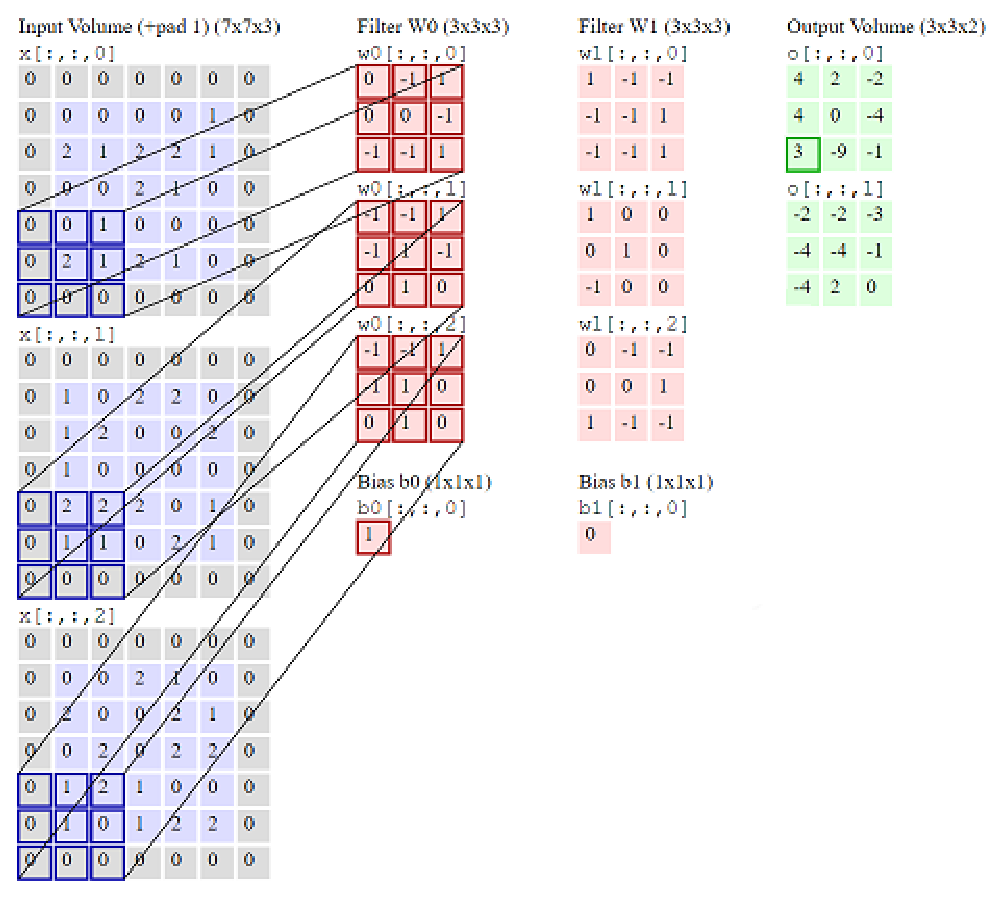
\includegraphics[width=0.8\textwidth,keepaspectratio]{figs/filter.eps}
    \caption{Two convolution computations~\cite{cs231} applied to an input (blue) of size $W=5$, filters (red) of size $F=3$, zero-padding (gray) $P=1$, and stride $S=2$. Through (\ref{eq:outsize}), we obtain the output matrix (green) height/width $(5-3+2\times 1)/2+1=3$ of depth two due to using two filters for an output shape $\in [3,3,2]$. The value $3$ is computed as the sum of all highlighted convolutions $x\circledast w0$, plus the bias $b0$.}
\label{fig:filter}      
\end{figure*}

Notice that the output volume is smaller than the input volume. A key role of zero-padding is to maintain dimension size throughout forward passes without adding information to the data. Stride can be set to one to capture the most information from each input, but can be set higher as a form of regularization, or to reduce computational complexity. The next difference is that a CNN applies its activation function as a separate layer, performing an element-wise function, leaving the output shape unchanged. A ReLU (\ref{eq:relu}) activation layer would maintain output shape, for example, computing each element $y=\max(0,x)$ from input element $x$.

A key operation CNNs perform is downsampling, which is often achieved by pool layers. Pool layers reduce the height/width of the current output shape by taking the population mean or max-valued element of a group of input values, governed by a filter size and stride, similarly to convolutional layers. This critical step has been shown~\cite{cs231} to reduce over-fitting while maintaining the key feature information of signals.

\begin{figure*}[ht!]
	\centering	\includegraphics[width=0.8\textwidth,keepaspectratio]{figs/pool.jpeg}
    \caption{Max pooling~\cite{cs231} of a 244 by 244 pixel image. Input size $W$ is 224, filter size $F$ is two, stride $S$ is two for an output shape (\ref{eq:outsize}) of $(224-2+2\times 0)/2+1=112$. Depth is maintained.}
\label{fig:pool}      
\end{figure*}

It has been found in practice that repeating sequences of convolutional and down-sampling layers can extract higher dimension features in signals and images~\cite{cs231}. CNN layer sequences are typically terminated with a few fully connected dense layers whose elements correspond to class scores. Consider the ConvNet CNN architecture in Figure~\ref{fig:convnet}.

\begin{figure*}[ht!]
	\centering	\includegraphics[width=0.8\textwidth,keepaspectratio]{figs/convnet.jpeg}
    \caption{A ConvNet architecture~\cite{cs231} that takes raw image pixel values as input, and outputs a five-element fully-connected layer, where each value corresponds to the CNN's belief that the raw image belongs to a label. In this case, the image is likely a car.}
\label{fig:convnet}      
\end{figure*}

There have been many investigations in the last decades into what the best CNN architectures are. There is a lot to decide, including where to place down-sampling, convolution, fully-connected, and activation layers, as well as how many sequences of those placements to use. Additionally, each process is dictated by potentially dozens of hyper-parameters. Below is a brief list of powerful, popular, and recent CNN architectures:
\begin{itemize}
\item LeNet~\cite{lenet} is the first successful CNN architecture, used to read zip codes and digits.
\item AlexNet~\cite{imagenet} is very similar to LeNet but is much deeper and more popular. Presented in 2012, AlexNet featured stacked convolutional layers, where previously such layers were always followed immediately by pooling layers.
\item ZFNet~\cite{zfnet} was presented in 2013 as an improvement to AlexNet, designing the middle convolutional layers to be bigger than the starting and ending ones. Additionally, hyper parameters were tweaked, making the stride and filter size of the first convolutional layer very small.
\item GoogLeNet~\cite{googlenet} was designed in 2014 by a group of staff from Google. The architecture made use of an Inception Module, reducing the number of parameters by an order of magnitude. Additionally, GoogLeNet found that the parameters contained in the ending fully-connected layers in previous CNNs did not have much impact on classification accuracy. By removing these and replacing the fully-connected layers with average-pooling layers, parameter counts can be further reduced.
\item VGGNet~\cite{vggnet} was also introduced in 2014, drawing attention to network depth. The optimal depth they found was having 16 layers, but the architecture is mostly popular for its very homogeneous composition of repeating 3x3 convolutional layers and 2x2 pooling layers from start to finish.
\item ResNet~\cite{resnet} was presented in 2015, featuring skip connections, batch normalization, and a complete lack of fully-connected layers. Skip connections helped SGD training (\ref{eq:gradient}) avoid gradient saturation, while batch normalization and a lack of fully-connected layers reduced training complexity.
\end{itemize}

\subsubsection{Regularization}
While pooling is an intuitive and computationally simple method of down-sampling, there are several other popular methods to control the capacity of a CNN to prevent over-fitting:
\begin{itemize}
\item L2 regularization adds the term $R(w)=\frac{1}{2}\lambda w^2$ to the loss function (\ref{eq:svmvector}). The $\frac{1}{2}$ constant is used such that the gradient calculated during SGD is equal to $\lambda w$. L2 regularization requires weight decay (see Section~\ref{linclass}: Parameter Updates) to be linear (or vanilla).
\item L1 regularization is similar to L2 regularization, often combined in the form $R(w) = \lambda_1 \mid w \mid + \lambda_2 w^2$. This combination is defined as elastic net regularization, resulting in most weights being near zero, causing the weight matrix to be sparse. Consequently, most parameters can be ignored, and only parameters corresponding to the strongest features need to be used.
\item Max norm constraints bound weight values by imposing the upper limit $\Vert \vec{w} \Vert_2 < c$. This prevents weights from significant increases, but adds ambiguity to weight information in cases where many weights are clamped.
\item Dropout~\cite{dropout} is the most effective and simple regularization method~\cite{cs231}. Dropout sets weights that connect any two layers to zero during training with probability $p$.
\end{itemize}

\begin{figure*}[ht!]
	\centering	\includegraphics[width=0.8\textwidth,keepaspectratio]{figs/dropout.jpeg}
    \caption{An illustration~\cite{cs231} of the last few layers of a linear classifier before (a) and after (b) dropout layers are implemented. Arrows represent connections between neurons, while neurons with x's through them represent neuron connections terminated by being dropped out.}
\label{fig:drop}      
\end{figure*}

\subsection{Novel Training Methods: Bayesian Optimization}
\label{bayesian}
Bayesian optimization\cite{bayesian} aims to find the global maximizer $x^*$ of the unknown objective function $f$ such that:
\begin{equation}
\label{eq:bayesianfun}
x^* = \argmax_{x\in \chi} f(x),
\end{equation}
where $\chi$ is the design space. Bayesian optimization has a bigger scope than neural networks. A CNN (see Section~\ref{cnn}) can be represented by the tunable parameters (weights) $W=x$ and the observed classification accuracy (loss function) $L=f$ (\textit{i.e.,} equation (\ref{eq:svmvector})). The reason for this is because Bayesian optimization is any sequential model-based approach to solving a problem. Updates to the parameters $x$ are provided via Bayesian posterior updates, or our updated beliefs given data. Posterior updates are guided by acquisition functions $\alpha_n : \chi$, where the next parameters in time $x_{n+1}$ are chosen by maximizing the current time acquisition function $\alpha_n$. To accomplish this goal, Bayesian optimization asks for two ingredients: a probabilistic surrogate model which contains a prior distribution, describing our current beliefs about the unknown loss function, and a known loss function that describes how optimal a series of queries are at accomplishing a task. The expected loss function is minimized to select the optimal queries, and the observed outputs cause the prior to be updated to provide a more accurate distribution.

Use of an acquisition function is often much more computationally expensive than optimizing the black box fucntion $f$, so it is critical that the acquisition functions be simple to evaluate. See Figure~\ref{fig:bayesianill} for an illustration of three time iterations of Bayesian optimization.

\begin{figure*}[ht!]
	\centering	\includegraphics[width=0.8\textwidth,keepaspectratio]{figs/bayesian.png}
    \caption{An illustration~\cite{bayesian} of three time iterations of (\ref{eq:bayesianfun}). The black line is the estimated objective or loss function $f$, while the dashed black line is the true $f$ (unknown but visualized). The acquisition function $\alpha$ is in green, whose maxima are highlighted with red arrows, indicating either exploration (when uncertainty $\sigma(\cdot)$, blue, is large) or exploitation (model prediction is high, solid and dashed black lines match). Observations $x_n$ are marked as black dots, with the new observations in the n=3 and n=4 sub-figures highlighted in red. Notice how new observations reduce uncertainty, and are first taken at high value points (right skewed) to maximize impact on acquisition function reduction.}
\label{fig:bayesianill}      
\end{figure*}

\subsubsection{Parametric Models}
Given an a priori distribution $p(w)$ which describes probable values for parameters $w$ before observing data, the a posteriori distribution $p(w | \mathcal{D})$ can be inferred using Bayes' rule:
\begin{equation}
\label{eq:bayesrule}
p(w | \mathcal{D}) = \frac{p(\mathcal{D} | w) p(w)}{p(\mathcal{D})},
\end{equation}
which describes our updated beliefs about $w$ after observing data $\mathcal{D}$. The choice of statistical model used now is paramount to the effectiveness of the Bayesian optimization~\cite{bayesian}. The simplest such model to perform Thompson Sampling in the Beta-Bernoulli Bandit Model. The metaphor the name is based on is a gambling one, where a bandit Bernoulli problem is considered. A slot machine has $K$ arms or levers, each with some probability of winning money. The effectiveness of each arm on the bandit is modeled as the function $f$, taking function input $a \in 1,...,K$, returning the Bernoulli parameter $\in (0,1)$. With the outcome of winning money or not denoted as $y_i \in \{0,1\}$, the outcome of pulling arm $a_i$ has mean parameter $f(a_i)$. With the $K$ arms available, $f$ can be fully described by parameters $w\in (0,1)^K$.

Once arms start getting pulled, it can be seen how often each arm actually wins money, and the comparison is made to probability the arm was believed to have to win money. This data is represented as $\mathcal{D} = \{(a_i,y_i)\}_{i=1}^n$, where $a_i$ indicates which of the $K$ arms were pulled, and $y_i$ is one of money was won and zero otherwise. We can compute the a posteriori distribution using the prior distribution over $w$:
\begin{equation}
\label{eq:betabandit}
p(w | \alpha, \beta) = \prod_{a=1}^{K} beta(w_a | \alpha,\beta),
\end{equation}
which is a good choice because beta distributions are the conjugate prior to the Bernoulli likelihood, or part of the same probability distribution family. For example, given the Bernoulli likelihood:
\begin{equation}
\label{eq:bernoulliex}
p(s) = {n\choose s}q^s(1-q)^{n-s},
\end{equation}
for $s$ successes, $n$ trials, and $q \in (0,1)$ the probability of success, the beta distribution conjugate prior describing the probabilities of which values $q$ can take can be described as:
\begin{equation}
\label{eq:betaex}
p(q) = \frac{q^{\alpha -1}(1-q)^{\beta -1}}{B(\alpha, \beta)}.
\end{equation}
Going back to the bandit statistical model, the a posteriori distribution can be derived using (\ref{eq:betabandit}) as:
\begin{equation}
\label{eq:posteriori}
p(w | \alpha, \beta) = \prod_{a=1}^{K} beta(w_a | \alpha+n_{a,1},\beta+n_{a,0}),
\end{equation}
where $n_{a,0} = \sum_{i=1}^n \mathbb{I}(y_i=0,a_i=a)$ is the number of losses resulting from pulling arm $a$ and $n_{a,1} = \sum_{i=1}^n \mathbb{I}(y_i=1,a_i=a)$ is the number of wins resulting from pulling arm $a$. The hyper-parameters $\alpha, \beta$ must be tuned. Finally, we decide the next arm $a_{n+1}$ to pull by posterior sampling a single sample $\tilde{w}$ from the posterior and maximizing the surrogate $f_{\tilde{w}}$:
\begin{equation}
\label{eq:picknextarm}
a_{n+1} = \argmax_a f_{\tilde{w}} (a), \tilde{w} \sim p(w|\mathcal{D}_n).
\end{equation}
Arms are only explored under this model if they are likely under the belief of the posterior to be optimal, or bring in the most wins. Using the bandit parametric model in deep learning, weights $W$ would be updated at each step $n$ in descending order from the most to least impact on reducing the loss function.

\subsubsection{Non-Parametric Models}
Can we make predictions on outcomes from arm-pulling without the parameters $w$? Using a kernel mapping trick, rather than mapping features to labels, we can describe a similarity between points, depending on which paradigm is more computationally tractable. In other words, it is simpler to work with the distances between points rather than to map those points in high-dimensional space. This requires only a $J \times J$ matrix inversion on kernels as opposed to the parametric models' $n \times n$ matrix of time indexed observation periods. Consider the following kernel model:
\begin{equation}
\label{eq:kernel}
K_{i,j} = k(x_i,x_j) = \Phi(x_i)V_0 \Phi(x_j)^T = \langle \Phi(x_i), \Phi(x_j) \rangle_{V_0},
\end{equation}
where $\Phi=\phi(X)$ is the feature mapping matrix on design matrix $X$, $V_0$ a hyper-parameter denoting the variance of a zero-mean Gaussian random variable, $x_{i,j}$ are all similar pairs of points in $X$, and $\langle \Phi(x_i), \Phi(x_j) \rangle_{V_0}$ is the inner product. The benefit of the kernel line of thinking is a normally distributed, data-driven posterior distribution can be described by mean and variance below, with no parameters known as a Gaussian Process:
\begin{subequations}
\label{eq:noparamposterior}
\begin{align}
\mu_n(x)=\mu_0(x)+k(x)^T(K+\sigma^2 I)^{-1} (y-m),
\\
\sigma_n^2(x)=\mathtt{k}(x,x)-k(x)^T(K+\sigma^2I)^{-1} k(x),
\end{align}
\end{subequations}
where $k(x)$ is the covariance between point $x$ and all previous observations, and $\mathtt{k}(x_i,x_j)$ is the kernel at $K_{i,j}$. The above mean and variance describe the non-parametric model's estimation and uncertainty at point $x$ representing the solid black line and blue uncertainty area in Figure~\ref{fig:bayesianill}, accomplished without weights $W$ but with kernels $K$. A simple and common kernel $\mathtt{k}(x,x')$ is the Mat\'ern~\cite{matern} stationary kernel covariance function:
\begin{equation}
\label{eq:matern}
\mathtt{k}(x,x') = \theta_0^2 \exp(-r),
\end{equation}
for $r^2= (x,x')^T \Lambda (x,x')$, and $\Lambda$ the diagonal matrix populated by $d$ length scales $\theta_i^2$. All $\theta$ values are hyper-parameters. This section only begins to scratch the surface of Bayeseian optimization. Besides the kernel above there is a host of other options, as well as many parametric and non-parametric methods such as linear models, sparse spectrum Gaussian Processes, Sparse Pseudo-input Gaussian Processes, and Random Forest. Finally there is a choice of acquisition functions not even covered here, although in~\cite{bayesian} it is mentioned that hyper-parameter and acquisition function choice does not have a strong impact on performance.

\subsection{Novel Training Methods: Distillation}
\label{distill}
Distillation is an idea\cite{distill} that begins with the thought that a very costly but effective way of improving a classifier's classification accuracy on a given signal would be to have many identical neural networks classify a signal and average the results, due to the random nature of SGD, SVM, or other training methods.

In Section~\ref{linclass}: Soft-Max Classifier, the soft-max function (\ref{eq:softmax}) was discussed in its use to describe a neural network's belief in a signal belonging to a class. What that equation leaves out is a scaling parameter named temperature, which determines how far or closely spaced probabilities are. Soft-max functions with high temperature tend towards equal probabilities, where low temperature soft-max functions tend to award the highest probability a value of one, all else zero. In its simplest form, distillation trains two neural networks, one with a low parameter count and one with a cumbersome, high parameter count, with high temperature $T$ in its soft-max:
\begin{equation}
\label{eq:tempsoftmax}
f_j(z) = \frac{e^{z_j/T}}{\sum_k e^{z_k/T}}.
\end{equation}
After training, the temperature is set to one in the distilled network, but kept constant in the cumbersome network. This high-entropy form of training has seen considerable investigation since the foundational paper~\cite{distill} for its increases in classification accuracy~\cite{distill} and increased security against adversarial perturbations~\cite{distdefense}.

\subsection{Novel Training Methods: Generative Adversarial Network (GAN)}
\label{gan}
Generative Adversarial Networks\cite{gan} achieve deep feature extraction on unannotated data through back passing through pairs of neural networks. Consider a decoy neural network that generates signals with the objective of fooling a modulation classifier CNN into thinking the signals it is observing are not of one modulation scheme, but another. It has been shown in many works~\cite{fooled} (see Figure~\ref{fig:fooled}) that small changes can be made to signals, images, and voice can render brittle classifiers useless.

\FloatBarrier
\begin{figure*}[ht!]
	\centering	\includegraphics[width=1\textwidth,keepaspectratio]{figs/diversity_40_images_label.png}
    \caption{A series of decoy images~\cite{fooled} fooling a computer vision classifier. Most images fail to remotely resemble their target label, however due to the brittle nature of training neural networks with standard back-pass techniques, small movements in feature-space at evaluation time can have significant and catastrophic results.}
\label{fig:fooled}      
\end{figure*}
\FloatBarrier

In a GAN setup, the decoy network described above is called the generator, while the modulation classifier is the discriminator. See Figure~\ref{fig:gan} for an overview of how networks in a GAN interact with each other.

\begin{figure*}[ht!]
	\centering	\includegraphics[width=0.8\textwidth,keepaspectratio]{figs/gan.png}
    \caption{A flow diagram~\cite{gan} of a GAN process. Synthetic data samples are added to data samples observed by the discriminator.}
\label{fig:gan}      
\end{figure*}

The essence of training a GAN is to find the parameters of the discriminator that maximize classification accuracy, and the parameters of the generator which minimize the discriminator's classification accuracy. For the generator, this means optimal parameters have been achieved when the discriminators accuracy falls to 0.5, or correctly classifying fake versus real samples half of the time. Given that there are only two labels, this accuracy is equal to that of a coin flip, or the best possible confusion.

\begin{figure*}[ht!]
	\centering	\includegraphics[width=0.8\textwidth,keepaspectratio]{figs/coregan.png}
    \caption{A flow diagram~\cite{gan} describing the SGD (\ref{eq:gradient}) feedback loop between the generator and discriminator (see Figure~\ref{fig:gan}). Parameter updates continue until the learning capacity of the networks are reached and classification accuracy of the discriminator reaches a steady state value $\in (0.5, 1)$.}
\label{fig:coregan}      
\end{figure*}

\subsection{Novel Training Methods: Domain Adaptation}
\label{domainadapt}
There is a method of generalized training~\cite{dadaptHRL} that has been explored in computer vision recently, motived by autonomous vehicle technology. There is not enough annotated (tagged with classification labels) images of roads environments, so a method was developed for training autonomous vehicle computer vision neural networks with computer-generated 3D images that still allow the networks to test well with real-world pictures at evaluation time (see Figure~\ref{fig:street}).

\begin{figure*}[ht!]
	\centering	\includegraphics[width=0.8\textwidth,keepaspectratio]{figs/street.png}
    \caption{A series of testing images and classification results~\cite{dadaptHRL}. A) Test image collected from real Cityscapes dataset. B) Identity mapped version of the image. C) Image translated to the target domain. D) Evaluation of translated image without domain adaptation. E) Evaluation of translated image using domain adaptation~\cite{dadaptHRL}. F) Translated image ground truth.}
\label{fig:street}      
\end{figure*}

The core idea of domain adaptation is to create a latent space $Z$ (see Figure~\ref{fig:adaptflow}) that is characteristic agnostic that can perform feature transformations on feature vectors learned from annotated data from the source domain $X$ into data from the target domain $Y$ using unannotated data from $Y$ such that a sum of weighted loss functions (see Figure~\ref{fig:adapt}) is minimized.

\begin{figure*}[ht!]
	\centering	\includegraphics[width=0.5\textwidth,keepaspectratio]{figs/domainadaptflow.png}
    \caption{A flow diagram~\cite{dadaptHRL} describing the various transforms $f_x, g_x, h, f_y, g_y$ and spaces $X$, $Z$, $Y$, $C$ and their interactions at the highest level in domain adaptation. The field is motivated by scarcity of annotated real pictures, but has much wider applications. Implemented correctly, training of classifiers becomes highly generalizable, making testing well under conditions not trained under becomes very robust when domain adaptation is performed on a set of unlabeled data from the new target domain.}
\label{fig:adaptflow}      
\end{figure*}

Domain adaptation attempts to perform SGD (\ref{eq:gradient}) on the general loss function
\begin{equation}
\label{eq:genloss}
Q = \lambda_cQ_c + \lambda_{id}Q_{id} + \lambda_zQ_z + \lambda_{tr}Q_{tr} + \lambda_{cyc}Q_{cyc} + \lambda_{trc}Q_{trc},
\end{equation}
where each individual loss function $Q$ is weighted by $\lambda$. Below, the role and contents of each loss function $Q$ is discussed.

\begin{itemize}
\item The core loss function $Q_c$ aims to perform the task of even the most basic linear classifier (see Section~\ref{linclass}): calculate some difference between each ground truth label $c_i$ and each evaluation signal. This is a standard neural net operation, independent from domain adaptation, described as~\cite{dadaptadversarial}:
\begin{equation}
\label{eq:qc}
Q_c = \sum_i l_c (h(f_x(x_i)),c_i),
\end{equation}
where $l_c$ is some loss function (\textit{i.e.,} $L_1$ norm, $L_2$ norm cross entropy), $h : Z \Rightarrow C$ is the transform in Figure~\ref{fig:adaptflow} from $Z$ space to the annotations $C$, and $x_i$ is a signal from the source domain $X$.
\item First and foremost in domain adaptation, it is desired for the transforms in Figure~\ref{fig:adaptflow} to only remove structured noise from signals, not information bits. The mapping from the $X$ or $Y$ domain to the $Z$ domain and back should be as close to an identity mapping as possible. That is the role of the individual loss function $Q_{id}$~\cite{drcn}, which is described as:
\begin{equation}
\label{eq:qid}
Q_{id} = \sum_i l_{id}(g_x(f_x(x_i)),x_i)+\sum_j l_{id}(g_y(f_y(y_j)),y_j),
\end{equation}
where $l_{id}$ is the sample or pixel-wise loss function (\textit{i.e.,} $L_1$ or $L_2$ norm).
\item Secondly, it is very important for the latent $Z$ space to be domain agnostic. This is achieved by training the $Z$ space using a GAN (see Section~\ref{gan}) discriminator $d_z : Z \rightarrow \{c_x,c_y \}$ ($c$ are annotations mapped to $Z$) which tries to classify if a feature in the latent space $Z$ was generated from the $X$ or $Y$ domain. The GAN's loss function contributing to (\ref{eq:genloss}) can be described as~\cite{dadaptagnostic}:
\begin{equation}
\label{eq:qz}
Q_z = \sum_i l_a(d_z)f_x(x_i)),c_x)+\sum_j l_a(d_z(f_y(y_j)),c_y),
\end{equation}
where $l_a$ is a suitable loss function for GANs.
\item As an extra precaution to make sure the transforms in Figure~\ref{fig:adaptflow} are consistent, discriminators in the source domain $d_x : X \rightarrow \{c_x,c_y \}$ and target domain $d_y : Y \rightarrow \{c_x,c_y \}$ are trained\cite{dadaptcyc} to classify whether a sample is fake (from the other domain) or real (from its own domain). The loss function minimized to accomplish this must match ground truths $c_x$ to signals from the $X$ domain mapped through the $Z$ domain and into the target $Y$ domain, and likewise for the ground truths $c_y$ of signals from the $Y$ domain:
\begin{equation}
\label{eq:qtr}
Q_{tr} = \sum_i l_a(d_y(g_y(f_x(x_i))),c_x)+\sum_j l_a(d_x(g_x(f_y(y_j))),c_y),
\end{equation}
\item Similarly to (\ref{eq:qid}), a cycle loss function\cite{dadaptcyc} was developed to ensure the mapping from any signal in the $X$ domain to the $Z$ domain, $Y$ domain, back to the $Z$ domain, and finally back to the $X$ domain is as similar as possible to the original image. The equivalent is added for images from the target $Y$ domain to formulate identity mappings through the use of:
\begin{equation}
\label{eq:qcyc}
Q_{cyc} = \sum_i l_{id}(g_x(f_y(g_y(f_x(x_i)))),x_i)+\sum_j l_{id}(g_y(f_x(g_x(f_y(y_j)))),y_j),
\end{equation}
\item Similarly to (\ref{eq:qc}), a translations loss function formulated in~\cite{dadaptHRL} is minimized such that classifications on signals additionally passed through the fake domain ($Y$ if the signal is from $X$, $X$ if the signal is from $Y$) are correct in the $Z$ domain when mapped to annotations $C$.
\begin{equation}
\label{eq:qtrc}
Q_{trc} = \sum_i l_c(h(f_y(g_y(f_x(x_i)))),c_i).
\end{equation}
\end{itemize}

\begin{figure*}[ht!]
	\centering	\includegraphics[width=1\textwidth,keepaspectratio]{figs/domainadapt.png}
    \caption{An elaborated~\cite{dadaptHRL} flow diagram of Figure~\ref{fig:adaptflow}, describing additionally the various weighted loss functions $Q_c, Q_{id}, Q_z, Q_{tr}, Q_{cyc}, Q_{trc}$ and how they interact with each domain $X$, $Y$, and $Z$. See equations (\ref{eq:qc}) through (\ref{eq:qtrc}).}
\label{fig:adapt}      
\end{figure*}

\section{Modulation Classification}
\label{modclass}
In Section~\ref{training}, Chapter~\ref{chapter3}, and Chapter~\ref{chapter4}, the concept of classification labels is often mentioned, and used in the context of modulation classification. The aim of this section is to communicate to the reader what a modulation scheme is, and the different forms neural nets take to classify them.
\subsection{Signal Modulation}
In the field of communications, a modulated signal $y(t)$ is simply the multiplication of the signal to be transmitted, $u(t)$, with a cosine described by $\omega_0$, its carrier frequency, $\cos(\omega_0 t)$.
\begin{equation}
\label{eq:modulate}
y(t) = u(t) \cos(\omega_0 t),
\end{equation}
and that signal is typically demodulated into a base-band signal $z(t)$ by the receiver chain through the use of a demodulator, which can be described as:
\begin{equation}
\label{eq:demodulate}
z(t) = u(t) \cos(\omega_0 t).
\end{equation}
However, this process has been shown~\cite{pahlavan2005wireless} to result in frequency-domain periodic copies of the signal in $z(\omega)$, so a low-pass filter $H(\omega)$ must be implemented to remove them.

\begin{figure*}[ht!]
	\centering	\includegraphics[width=1\textwidth,keepaspectratio]{figs/txrx.png}
    \caption{A very high-level flow diagram~\cite{mods} describing the flow of information in a communications transmit-receive pair. Information begins as bits mapped to IQ points, is transformed into a voltage by a DAC, transduced into an electromagnetic wave by a transmitting antenna, travels through a noisy channel, is transduced back into a voltage by a receiving antenna, detected and transformed into IQ points with the help of a ADC, and finally mapped back to bits.}
\label{fig:txrx}      
\end{figure*}

A primary use of signal modulation is traffic control. Two signals being sent by two transmit-receive pairs in the same location at the same time can be clearly detected and recovered~\cite{pahlavan2005wireless} when modulated differently, or using the same scheme at different carrier frequencies. Another key benefit of modulation is to reduce the corruption of signals when traveling through a noisy channel~\cite{rappaport1996wireless}.

\subsubsection{Designing a Modulation Scheme}
While an exhaustive list of modulation schemes and their performance can be found in~\cite{mods}, the design and use of the Quadrature Phase Shift Keying (QPSK) modulation scheme is described in this section to give a better idea behind modulation scheme use.

Typically modulation schemes are described as being $M-ary$, or having $M$ unique constellation points. For information represented by a number of bits $b$, $M$ is calculated as:
\begin{equation}
\label{eq:mary}
2^b = M.
\end{equation}
Modulation schemes are typically expressed as $s_n(t)$, time domain cosines that are functions of the message, $n$. In the case of QPSK $M = 4 = 2^b$ for $b = \log_2(M) = 2$, meaning each message contains two bits of information. Each possible message $n=1,2,3,4$ represents the binary message transform $n = i : b \rightarrow (b_1, b_2), i=1,2,3,4$, resulting in $n=1 : b \rightarrow (0, 0) = 0, n=2 : b \rightarrow (0, 1), n=3 : b \rightarrow (1, 0)$, and $n=4 : b \rightarrow (1, 1)$. For QPSK, the constellation map $s_n(t)$ is described as:
\begin{equation}
\label{eq:qpsk}
s_n(t) = \sqrt{\frac{2 E_s}{T_s}} \cos(2\pi f_c t + (2n-1)\frac{\pi}{4}), n=1,2,3,4,
\end{equation}
where $E_s$ is the energy in Joules per symbol $n = i : b \rightarrow (b_1, b_2), i=1,2,3,4$, $T_s$ is the sampling period of the ADC/DAC in Hz, and $f_c$ is the modulation carrier frequency. It can be shown that any modulation constellation can be represented by a set of basis functions and amplitudes $s_n(t)=s_{n1} \phi_1(t) + s_{n2} \phi_2(t)$. Basis functions must be orthogonal, and the whole set orthonormal, meaning each basis is a vector in euclidean space on a unique axis of the coordinate space, mathematically defined as the inner product of any two basis functions being zero $\langle \phi_i(t), \phi_j(t) \rangle = \int_0^T \phi_i(t) \phi_j(t) = 0$.For QPSK, these are derived~\cite{rappaport1996wireless}:
\begin{subequations}
\label{eq:basisfun}
\begin{align}
\phi_1(t) = \sqrt{\frac{2}{T_s}} \cos(2\pi f_c t),
\\
\phi_2(t) = \sqrt{\frac{2}{T_s}} \sin(2\pi f_c t),
\end{align}
\end{subequations}
resulting in the points $\big(\pm \sqrt{E_s/2}, \pm \sqrt{E_s/2} \big)$ for $n=1,2,3,4$, shown in Figure~\ref{fig:qpskconst}.
\begin{figure*}[ht!]
	\centering	\includegraphics[width=0.8\textwidth,keepaspectratio]{figs/qpsk.png}
    \caption{A set of QPSK constellation points (\ref{eq:qpsk}) for $E_s=4$. The horizontal axis is defined as $\phi_1(t)$ or the real valued element in a complex tuple, and the vertical axis as $\phi_2(t)$, traditionally represented as the imaginary valued element in a complex tuple. The resulting transformations are $n = 1 : b\rightarrow (0, 0) : s \rightarrow (2/\sqrt{2}, 2/\sqrt{2})$, $n = 2 : b\rightarrow (0, 1) : s \rightarrow (-2/\sqrt{2}, 2/\sqrt{2})$, $n = 3 : b\rightarrow (1, 0) : s \rightarrow (-2/\sqrt{2}, -2/\sqrt{2})$, and $n = 4 : b\rightarrow (1, 1) : s \rightarrow (2/\sqrt{2}, -2/\sqrt{2})$}
\label{fig:qpskconst}      
\end{figure*}
A common metric used to describe the effectiveness of any given modulation scheme is its efficiency $\epsilon_p$, defined as the squared minimum euclidean distance between any two constellation points $s_n(t)$, divided by the population mean energy in Joules per bit.
\begin{equation}
\label{eq:modeff}
\epsilon_p = \frac{d_{min}^2}{\bar{E}_b}
\end{equation}
For the case of QPSK, there are two bits per symbol, so $\bar{E}_b = \frac{1}{2}\bar{E}_s$. For (\ref{eq:basisfun}), the $L_2$ norm of the basis functions is $d_{min}^2 = \int_0^T (\phi_1(t) - \phi_2(t))^2 dt = ||s_1(t) - s_2(t)||^2 = (2/\sqrt{2}+2/\sqrt{2})^2 = 8$, $s_1(t), s_2(t)$ chosen since all points are equidistant. The energy per symbol is $\bar{E}_s = \langle s_1(t), s_1(t) \rangle = (2/\sqrt{2})^2 + (2/\sqrt{2})^2 = 4$, so the efficiency comes out to be $\epsilon_p = 8/(4/2) = 4$, which is the highest efficiency a modulation scheme can achieve when using all constellation points available~\cite{rappaport1996wireless}.

\subsection{Modulation Classification}
In a communications transmit receive pair, it is not always known a priori which modulation scheme is to be used. This can cause critical failure, as if an incoming signal cannot be properly mapped to the right message bits, bit error rate can increase significantly. Although numerous~\cite{modclassback} Automatic Modulation Classification (AMC) methods have existed for decades, the area has seen new life with the data-driven, high accuracy classification results coming in from new deep neural networks~\cite{modclassback}. It is the goal of this section to investigate the architecture of a foundational~\cite{modclassback} Convolutional Long short-term Deep Neural Network (CLDNN) that performs modulation classification, as to provide insight on what is happening behind-the scenes when modulation classification is mentioned in other parts of this work.

In~\cite{modclassback}, signals $x_i \in [2, 128]$ are defined by two rows for in-phase and quadrature components, and 128 columns for each complex sample. The architecture used is exceedingly simple: two convolutional layers (see Section~\ref{cnn}) and a single dense layer followed by a soft-max (\ref{eq:softmax}) classifier. The hidden layers are followed by ReLU (\ref{eq:relu}) activation layers, and dropout layers (see Figure~\ref{fig:drop}) with $p=0.5$. In~\cite{modclassback} figures describing their optimization process are detailed, resulting in choosing a filter size $F=8$, stride $S=1$, and 50 filters (see Figure~\ref{fig:filter} for an example convolution).

\begin{figure*}[ht!]
	\centering	\includegraphics[width=1\textwidth,keepaspectratio]{figs/cldnn.png}
    \caption{A flow chart~\cite{modclassback} describing the forward pass (see Figure~\ref{fig:relucircuit}) of a set of eight input values through the CLDNN. A $[1,8]$ input vector is concatenated with values filtered through a $[1,8]$ filter in both the first and second convolutional layer. Each filter (see Figure~\ref{fig:filtresp}) contains eight weights and one bias value (see Figure~\ref{fig:filter} for example filters), which are calculated during SGD (\ref{eq:gradient}). The Long Short-Term Memory (LSTM) cell holds the values for the soft-max classification layer.}
\label{fig:cldnn}      
\end{figure*}

\begin{figure*}[ht!]
	\centering	\includegraphics[width=0.7\textwidth,keepaspectratio]{figs/train_sig.png}
    \caption{The time-domain IQ plot~\cite{modclassback} of a $[2,128]$ output signal from the $[1,8]$ filter in Figure~\ref{fig:filtresp}. The signal input to the filter was random, but trained to maximally activate the filters eight weights. The result is a Binary Phase Shift Keying (BPSK) waveform, indicating that this filter was trained to maximize the eventual soft-max class scores of BPSK signals.}
\label{fig:trainsig}      
\end{figure*}

\begin{figure*}[ht!]
	\centering	\includegraphics[width=0.7\textwidth,keepaspectratio]{figs/filter_resp.png}
    \caption{Time (top) and frequency (bottom) domain magnitude plots~\cite{modclassback} of a trained $[1,8]$ filter like those in Figure~\ref{fig:cldnn}. This filter's first, second, and seventh weights have the most influence on classification. See Figure~\ref{fig:trainsig} for another visualization of this filter.}
\label{fig:filtresp}      
\end{figure*}

A common metric in modulation classification used to evaluate, in detail, the performance of a classifier is the confusion matrix, which simply describes how correctly a function answers different questions. The CLDNN in~\cite{modclassback} calculates a confusion matrix in Figure~\ref{fig:confmodclass}.
\FloatBarrier
\begin{figure*}[ht!]
	\centering	\includegraphics[width=0.7\textwidth,keepaspectratio]{figs/conf.png}
    \caption{A confusion matrix~\cite{modclassback} describing the classification accuracy of the CLDNN on all test signals at evaluation time. The color gradient communicates classification accuracy averaged over SNR values ranging from -20 dB to 20dB. The horizontal axis displays the modulation scheme that the CLDNN classifies signals by, and the vertical axis the ground truth of those signals. A perfectly performing classifier would have a deep brown diagonal matrix, where each signal of each modulation type of each SNR is correctly classified by having the highest soft-max value at its index corresponding to the signals' ground truth label.}
\label{fig:confmodclass}      
\end{figure*}
\FloatBarrier
\section{Summary}
In this chapter, various classical models for transmission imperfections and channel models were surveyed in Section~\ref{chanmods}. In Section~\ref{training}, the fundamentals of deep learning was discussed, specifically topics concerning training. Finally, Section~\ref{modclass} presented a survey of modulation classification, the primary form of neural network evaluation discussed in this thesis.

In the next Chapter~\ref{chapter3}, a novel framework for low-decay, low-bias dataset generation is presented.\\
